% Options for packages loaded elsewhere
% Options for packages loaded elsewhere
\PassOptionsToPackage{unicode}{hyperref}
\PassOptionsToPackage{hyphens}{url}
\PassOptionsToPackage{dvipsnames,svgnames,x11names}{xcolor}
%
\documentclass[
  letterpaper,
  DIV=11,
  numbers=noendperiod]{scrartcl}
\usepackage{xcolor}
\usepackage[margin=1in]{geometry}
\usepackage{amsmath,amssymb}
\setcounter{secnumdepth}{5}
\usepackage{iftex}
\ifPDFTeX
  \usepackage[T1]{fontenc}
  \usepackage[utf8]{inputenc}
  \usepackage{textcomp} % provide euro and other symbols
\else % if luatex or xetex
  \usepackage{unicode-math} % this also loads fontspec
  \defaultfontfeatures{Scale=MatchLowercase}
  \defaultfontfeatures[\rmfamily]{Ligatures=TeX,Scale=1}
\fi
\usepackage{lmodern}
\ifPDFTeX\else
  % xetex/luatex font selection
\fi
% Use upquote if available, for straight quotes in verbatim environments
\IfFileExists{upquote.sty}{\usepackage{upquote}}{}
\IfFileExists{microtype.sty}{% use microtype if available
  \usepackage[]{microtype}
  \UseMicrotypeSet[protrusion]{basicmath} % disable protrusion for tt fonts
}{}
\makeatletter
\@ifundefined{KOMAClassName}{% if non-KOMA class
  \IfFileExists{parskip.sty}{%
    \usepackage{parskip}
  }{% else
    \setlength{\parindent}{0pt}
    \setlength{\parskip}{6pt plus 2pt minus 1pt}}
}{% if KOMA class
  \KOMAoptions{parskip=half}}
\makeatother
% Make \paragraph and \subparagraph free-standing
\makeatletter
\ifx\paragraph\undefined\else
  \let\oldparagraph\paragraph
  \renewcommand{\paragraph}{
    \@ifstar
      \xxxParagraphStar
      \xxxParagraphNoStar
  }
  \newcommand{\xxxParagraphStar}[1]{\oldparagraph*{#1}\mbox{}}
  \newcommand{\xxxParagraphNoStar}[1]{\oldparagraph{#1}\mbox{}}
\fi
\ifx\subparagraph\undefined\else
  \let\oldsubparagraph\subparagraph
  \renewcommand{\subparagraph}{
    \@ifstar
      \xxxSubParagraphStar
      \xxxSubParagraphNoStar
  }
  \newcommand{\xxxSubParagraphStar}[1]{\oldsubparagraph*{#1}\mbox{}}
  \newcommand{\xxxSubParagraphNoStar}[1]{\oldsubparagraph{#1}\mbox{}}
\fi
\makeatother

\usepackage{color}
\usepackage{fancyvrb}
\newcommand{\VerbBar}{|}
\newcommand{\VERB}{\Verb[commandchars=\\\{\}]}
\DefineVerbatimEnvironment{Highlighting}{Verbatim}{commandchars=\\\{\}}
% Add ',fontsize=\small' for more characters per line
\usepackage{framed}
\definecolor{shadecolor}{RGB}{241,243,245}
\newenvironment{Shaded}{\begin{snugshade}}{\end{snugshade}}
\newcommand{\AlertTok}[1]{\textcolor[rgb]{0.68,0.00,0.00}{#1}}
\newcommand{\AnnotationTok}[1]{\textcolor[rgb]{0.37,0.37,0.37}{#1}}
\newcommand{\AttributeTok}[1]{\textcolor[rgb]{0.40,0.45,0.13}{#1}}
\newcommand{\BaseNTok}[1]{\textcolor[rgb]{0.68,0.00,0.00}{#1}}
\newcommand{\BuiltInTok}[1]{\textcolor[rgb]{0.00,0.23,0.31}{#1}}
\newcommand{\CharTok}[1]{\textcolor[rgb]{0.13,0.47,0.30}{#1}}
\newcommand{\CommentTok}[1]{\textcolor[rgb]{0.37,0.37,0.37}{#1}}
\newcommand{\CommentVarTok}[1]{\textcolor[rgb]{0.37,0.37,0.37}{\textit{#1}}}
\newcommand{\ConstantTok}[1]{\textcolor[rgb]{0.56,0.35,0.01}{#1}}
\newcommand{\ControlFlowTok}[1]{\textcolor[rgb]{0.00,0.23,0.31}{\textbf{#1}}}
\newcommand{\DataTypeTok}[1]{\textcolor[rgb]{0.68,0.00,0.00}{#1}}
\newcommand{\DecValTok}[1]{\textcolor[rgb]{0.68,0.00,0.00}{#1}}
\newcommand{\DocumentationTok}[1]{\textcolor[rgb]{0.37,0.37,0.37}{\textit{#1}}}
\newcommand{\ErrorTok}[1]{\textcolor[rgb]{0.68,0.00,0.00}{#1}}
\newcommand{\ExtensionTok}[1]{\textcolor[rgb]{0.00,0.23,0.31}{#1}}
\newcommand{\FloatTok}[1]{\textcolor[rgb]{0.68,0.00,0.00}{#1}}
\newcommand{\FunctionTok}[1]{\textcolor[rgb]{0.28,0.35,0.67}{#1}}
\newcommand{\ImportTok}[1]{\textcolor[rgb]{0.00,0.46,0.62}{#1}}
\newcommand{\InformationTok}[1]{\textcolor[rgb]{0.37,0.37,0.37}{#1}}
\newcommand{\KeywordTok}[1]{\textcolor[rgb]{0.00,0.23,0.31}{\textbf{#1}}}
\newcommand{\NormalTok}[1]{\textcolor[rgb]{0.00,0.23,0.31}{#1}}
\newcommand{\OperatorTok}[1]{\textcolor[rgb]{0.37,0.37,0.37}{#1}}
\newcommand{\OtherTok}[1]{\textcolor[rgb]{0.00,0.23,0.31}{#1}}
\newcommand{\PreprocessorTok}[1]{\textcolor[rgb]{0.68,0.00,0.00}{#1}}
\newcommand{\RegionMarkerTok}[1]{\textcolor[rgb]{0.00,0.23,0.31}{#1}}
\newcommand{\SpecialCharTok}[1]{\textcolor[rgb]{0.37,0.37,0.37}{#1}}
\newcommand{\SpecialStringTok}[1]{\textcolor[rgb]{0.13,0.47,0.30}{#1}}
\newcommand{\StringTok}[1]{\textcolor[rgb]{0.13,0.47,0.30}{#1}}
\newcommand{\VariableTok}[1]{\textcolor[rgb]{0.07,0.07,0.07}{#1}}
\newcommand{\VerbatimStringTok}[1]{\textcolor[rgb]{0.13,0.47,0.30}{#1}}
\newcommand{\WarningTok}[1]{\textcolor[rgb]{0.37,0.37,0.37}{\textit{#1}}}

\usepackage{longtable,booktabs,array}
\usepackage{calc} % for calculating minipage widths
% Correct order of tables after \paragraph or \subparagraph
\usepackage{etoolbox}
\makeatletter
\patchcmd\longtable{\par}{\if@noskipsec\mbox{}\fi\par}{}{}
\makeatother
% Allow footnotes in longtable head/foot
\IfFileExists{footnotehyper.sty}{\usepackage{footnotehyper}}{\usepackage{footnote}}
\makesavenoteenv{longtable}
\usepackage{graphicx}
\makeatletter
\newsavebox\pandoc@box
\newcommand*\pandocbounded[1]{% scales image to fit in text height/width
  \sbox\pandoc@box{#1}%
  \Gscale@div\@tempa{\textheight}{\dimexpr\ht\pandoc@box+\dp\pandoc@box\relax}%
  \Gscale@div\@tempb{\linewidth}{\wd\pandoc@box}%
  \ifdim\@tempb\p@<\@tempa\p@\let\@tempa\@tempb\fi% select the smaller of both
  \ifdim\@tempa\p@<\p@\scalebox{\@tempa}{\usebox\pandoc@box}%
  \else\usebox{\pandoc@box}%
  \fi%
}
% Set default figure placement to htbp
\def\fps@figure{htbp}
\makeatother

\ifLuaTeX
  \usepackage{luacolor}
  \usepackage[soul]{lua-ul}
\else
  \usepackage{soul}
\fi

% definitions for citeproc citations
\NewDocumentCommand\citeproctext{}{}
\NewDocumentCommand\citeproc{mm}{%
  \begingroup\def\citeproctext{#2}\cite{#1}\endgroup}
\makeatletter
 % allow citations to break across lines
 \let\@cite@ofmt\@firstofone
 % avoid brackets around text for \cite:
 \def\@biblabel#1{}
 \def\@cite#1#2{{#1\if@tempswa , #2\fi}}
\makeatother
\newlength{\cslhangindent}
\setlength{\cslhangindent}{1.5em}
\newlength{\csllabelwidth}
\setlength{\csllabelwidth}{3em}
\newenvironment{CSLReferences}[2] % #1 hanging-indent, #2 entry-spacing
 {\begin{list}{}{%
  \setlength{\itemindent}{0pt}
  \setlength{\leftmargin}{0pt}
  \setlength{\parsep}{0pt}
  % turn on hanging indent if param 1 is 1
  \ifodd #1
   \setlength{\leftmargin}{\cslhangindent}
   \setlength{\itemindent}{-1\cslhangindent}
  \fi
  % set entry spacing
  \setlength{\itemsep}{#2\baselineskip}}}
 {\end{list}}
\usepackage{calc}
\newcommand{\CSLBlock}[1]{\hfill\break\parbox[t]{\linewidth}{\strut\ignorespaces#1\strut}}
\newcommand{\CSLLeftMargin}[1]{\parbox[t]{\csllabelwidth}{\strut#1\strut}}
\newcommand{\CSLRightInline}[1]{\parbox[t]{\linewidth - \csllabelwidth}{\strut#1\strut}}
\newcommand{\CSLIndent}[1]{\hspace{\cslhangindent}#1}



\setlength{\emergencystretch}{3em} % prevent overfull lines

\providecommand{\tightlist}{%
  \setlength{\itemsep}{0pt}\setlength{\parskip}{0pt}}



 


\usepackage{booktabs}
\usepackage{longtable}
\usepackage{array}
\usepackage{multirow}
\usepackage{wrapfig}
\usepackage{float}
\usepackage{colortbl}
\usepackage{pdflscape}
\usepackage{tabu}
\usepackage{threeparttable}
\usepackage{threeparttablex}
\usepackage[normalem]{ulem}
\usepackage{makecell}
\usepackage{xcolor}
\KOMAoption{captions}{tableheading}
\makeatletter
\@ifpackageloaded{tcolorbox}{}{\usepackage[skins,breakable]{tcolorbox}}
\@ifpackageloaded{fontawesome5}{}{\usepackage{fontawesome5}}
\definecolor{quarto-callout-color}{HTML}{909090}
\definecolor{quarto-callout-note-color}{HTML}{0758E5}
\definecolor{quarto-callout-important-color}{HTML}{CC1914}
\definecolor{quarto-callout-warning-color}{HTML}{EB9113}
\definecolor{quarto-callout-tip-color}{HTML}{00A047}
\definecolor{quarto-callout-caution-color}{HTML}{FC5300}
\definecolor{quarto-callout-color-frame}{HTML}{acacac}
\definecolor{quarto-callout-note-color-frame}{HTML}{4582ec}
\definecolor{quarto-callout-important-color-frame}{HTML}{d9534f}
\definecolor{quarto-callout-warning-color-frame}{HTML}{f0ad4e}
\definecolor{quarto-callout-tip-color-frame}{HTML}{02b875}
\definecolor{quarto-callout-caution-color-frame}{HTML}{fd7e14}
\makeatother
\makeatletter
\@ifpackageloaded{caption}{}{\usepackage{caption}}
\AtBeginDocument{%
\ifdefined\contentsname
  \renewcommand*\contentsname{Table of contents}
\else
  \newcommand\contentsname{Table of contents}
\fi
\ifdefined\listfigurename
  \renewcommand*\listfigurename{List of Figures}
\else
  \newcommand\listfigurename{List of Figures}
\fi
\ifdefined\listtablename
  \renewcommand*\listtablename{List of Tables}
\else
  \newcommand\listtablename{List of Tables}
\fi
\ifdefined\figurename
  \renewcommand*\figurename{Figure}
\else
  \newcommand\figurename{Figure}
\fi
\ifdefined\tablename
  \renewcommand*\tablename{Table}
\else
  \newcommand\tablename{Table}
\fi
}
\@ifpackageloaded{float}{}{\usepackage{float}}
\floatstyle{ruled}
\@ifundefined{c@chapter}{\newfloat{codelisting}{h}{lop}}{\newfloat{codelisting}{h}{lop}[chapter]}
\floatname{codelisting}{Listing}
\newcommand*\listoflistings{\listof{codelisting}{List of Listings}}
\makeatother
\makeatletter
\makeatother
\makeatletter
\@ifpackageloaded{caption}{}{\usepackage{caption}}
\@ifpackageloaded{subcaption}{}{\usepackage{subcaption}}
\makeatother
\usepackage{bookmark}
\IfFileExists{xurl.sty}{\usepackage{xurl}}{} % add URL line breaks if available
\urlstyle{same}
\hypersetup{
  pdftitle={Report on the use of passive acoustic monitoring for analysis of bird trends in Jasper National Park},
  pdfauthor={Alex MacPhail; Brenda Shepherd; Nina Veselka},
  colorlinks=true,
  linkcolor={blue},
  filecolor={Maroon},
  citecolor={Blue},
  urlcolor={Blue},
  pdfcreator={LaTeX via pandoc}}


\title{Report on the use of passive acoustic monitoring for analysis of
bird trends in Jasper National Park}
\author{Alex MacPhail \and Brenda Shepherd \and Nina Veselka}
\date{2026-02-15}
\begin{document}
\maketitle

\renewcommand*\contentsname{Table of contents}
{
\hypersetup{linkcolor=}
\setcounter{tocdepth}{3}
\tableofcontents
}

\begin{center}
\pandocbounded{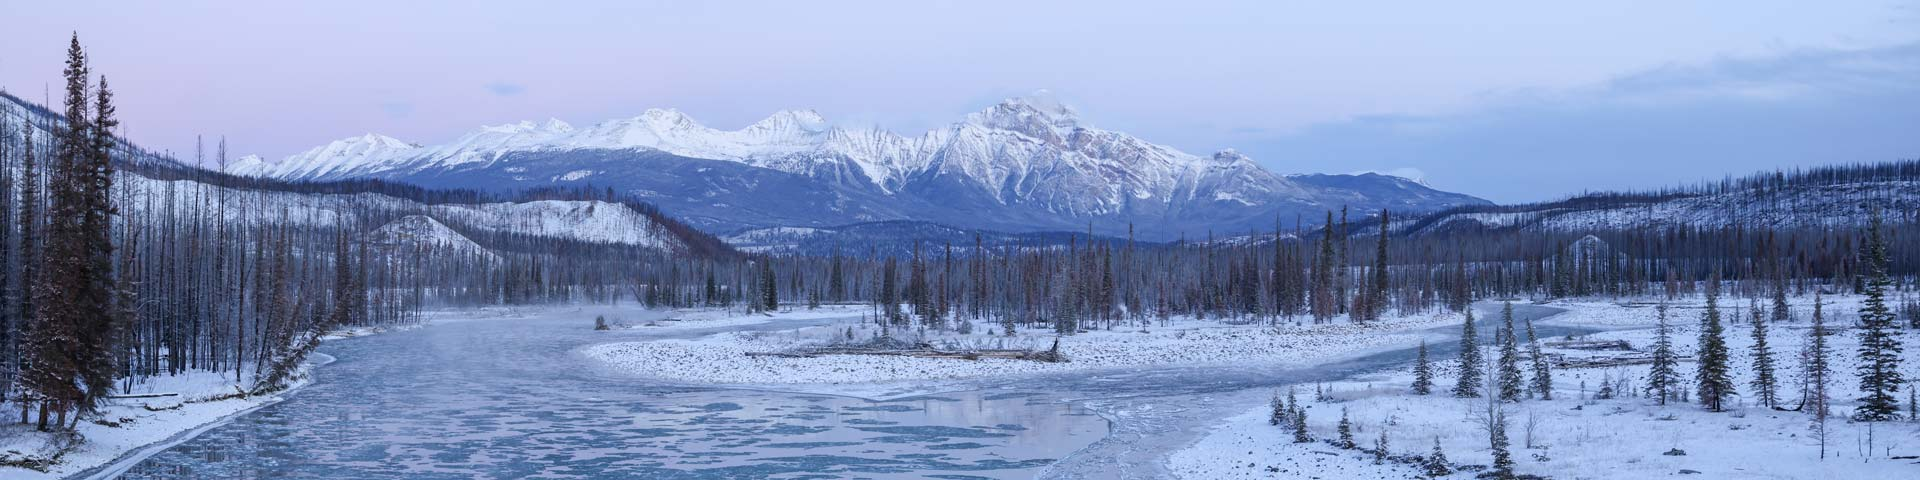
\includegraphics[keepaspectratio]{assets/janp.png}}
\end{center}

\begin{tcolorbox}[enhanced jigsaw, toptitle=1mm, title=\textcolor{quarto-callout-note-color}{\faInfo}\hspace{0.5em}{Note}, colback=white, colbacktitle=quarto-callout-note-color!10!white, opacitybacktitle=0.6, breakable, rightrule=.15mm, coltitle=black, toprule=.15mm, titlerule=0mm, left=2mm, bottomtitle=1mm, bottomrule=.15mm, arc=.35mm, leftrule=.75mm, opacityback=0, colframe=quarto-callout-note-color-frame]

This report is dynamically generated, meaning its results may evolve
with the addition of new data or further analyses. For the most recent
updates, refer to the publication date and feel free to reach out to the
authors.

\end{tcolorbox}

\section{Abstract}\label{abstract}

Since 2007, Jasper National Park has conducted passive acoustic
monitoring as part of its ecological integrity monitoring program. The
18 years of data were analyzed to identify trends and extract insights
that inform ongoing monitoring and strengthen future species monitoring
practices. The analysis assessed whether species and guild abundances
shifted by ±2.5\% in the alpine and montane ecoregions. Data were
managed and processed in WildTrax, combining and harmonizing legacy
datasets from multiple methodologies. Sampling locations were tested for
independence, and trend analyses quantified changes in species counts
over time across guilds and ecoregions.

\section{Land Acknowledgement}\label{land-acknowledgement}

We respectfully acknowledge that Jasper National Park is located in
Treaty 6 and 8 as well as the traditional lands of the Anishinabe,
Aseniwuche Winewak, Dene-zaa, Nêhiyawak, Secwépemc, Stoney Nakoda,
Mountain Métis and Métis. We acknowledge the past, present, and future
generations of these nations who continue to steward the land.

\section{Introduction}\label{introduction}

Human activities have been identified as key pressures and contributors
to the global decline in forest wildlife (Allan et al. (2017)). The
repercussions of habitat fragmentation (Fahrig (2003)) and loss (Hanski
(2011)), climate change (Mantyka-pringle, Martin, and Rhodes (2012),
Sattar et al. (2021), Abrahms et al. (2023)), and increased access to
sensitive areas exert direct and indirect pressures on forest
biodiversity, particularly in protected areas in Canada (Lemieux et al.
(2011)). In Alberta's Rocky Mountain Natural Region, these pressures are
compounded by increasing wildfire activity, which has significantly
impacted montane bird monitoring. Studies have shown large declines in
bird abundance in the last several decades across large regions of North
America (Rosenberg et al. (2019)), suggesting the need for parkwide
monitoring of bird abundance.

In 2007, Jasper National Park initiated a program incorporating passive
acoustic monitoring of the park's vocalizing wildlife. Autonomous
Recording Units (ARUs) are compact environmental sensors that are
designed to passively record the environment (Shonfield and Bayne
(2017)), capturing vocalizing species like birds and amphibians---a
method growing in use across the globe (Sugai et al. (2018)). This
technology enables biologists to conduct prolonged surveys with minimal
human interference, while creating a permanent, archiveable recording of
the soundscape. Given the rapidity and ease of accumulating data from
these units, maintaining a high standard of data integrity is paramount
to ensure future data interoperability and sharing. The data collected
by these units contribute valuable information to ecological integrity
metrics such as species richness, diversity, occupancy, abundance trends
of species and human activities in National Parks over time.

This project analyzes Jasper's passive acoustic monitoring data from
2007 to 2025, to assess trends while accounting for the clustering of
survey points within transects and determining time-to-first-detection
usability in analysis. We selected species abundance as our primary
monitoring measure following recommendations in \hl{Fletcher et
al.~(2025)}. Measures that reflect abundance, reproductive performance,
survival, dispersal, habitat quality, and role in ecosystem functioning
provide richer insights for the achievement of conservation goals than
species richness or species incidence. For example, incidence alone does
not mean that a species' presence is meaningful from a conservation
perspective because a single observation is treated the same as an
abundant species. As changes in abundance are more closely linked to
extinction risk than species incidence, abundance-based metrics have
been promoted to better assess goals in biodiversity conservation.
Abundance can fluctuate more than occurrence and may therefore better
track key changes in the environment, although care should be taken to
not overinterpret ``noisy'' abundance variation. Information on
abundance is essential for diagnosing decline and recovery of species
and may better capture the resilience of biodiversity to ongoing
environmental threats

Jasper National Park reports on the condition of three park ecosystems
in its State of the Park Report: freshwater, alpine and forest
(montane). Since birds are indicators in both the forest and alpine
ecosystems, separate analyses were conducted for the montane ecoregion
(grouping of the upper subalpine, lower subalpine, and true montane
ecoregions) and alpine ecoregion. To enhance accessibility and
reproducibility, the findings were presented in this online report with
fully documented code, allowing future updates as data collection
methods become standardized. Additionally, recommendations were
developed to refine data transcription priorities, improve annual
reporting methods, and evaluate species guild classifications for
long-term monitoring.

This project aims to analyze Jasper's passive acoustic monitoring data
from 2007 to 2025, assessing trends in species and guild abundance while
accounting for the clustering of survey points within transects.
Separate analyses will be conducted for montane and sub-alpine and
alpine ecoregions to align with Ecological Integrity reporting
requirements, determining time-to-first-detection usability in analysis.
To enhance accessibility and reproducibility, the findings will be
presented in this online report with fully documented code, allowing
future updates as data collection methods become standardized.
Additionally, recommendations will be developed to refine data
transcription priorities, improve annual reporting methods, and evaluate
species guild classifications for long-term monitoring. The objectives
of this report are to:

\begin{itemize}
\tightlist
\item
  Describe the data management and processing procedures for acoustic
  data collected from 2007 to 2025.
\item
  Compare how different data processing methods influence the count of
  species and individuals detected on recordings.
\item
  Report on trends in bird abundance by species and by guild in the
  montane (forest indicator) and alpine (alpine indicator) ecoregions,
  incorporating time-to-first-detection analysis

  \begin{itemize}
  \tightlist
  \item
    Summarize results by ecoregion as the percentage of species and
    guilds declining by ≥2.5\% in both forest and alpine regions.
    Explore methods (e.g., inclusion of covariates and summarizing by
    guild) to interpret these changes, understanding how birds may be
    responding to stressors in the park or across their ranges and how
    changing populations may affect ecosystems.
  \end{itemize}
\item
  Estimate species richness trends to determine if they provides insight
  about bird community conditions.
\item
  Provide recommendations for:

  \begin{itemize}
  \tightlist
  \item
    Prioritizing previous years' data for re-transcription to 1SPT;
  \item
    Optimizing annual reporting methods (e.g., baseline comparisons
    vs.~10-year trends); and
  \item
    Refining methods for evaluating species trends against thresholds
    and reviewing guilds and traits used in assessments
  \end{itemize}
\item
  Facilitate data publication to the public, resource managers, academic
  institutions, and any other relevant agencies
\end{itemize}

\section{Methods}\label{methods}

\subsection{Bird surveys}\label{bird-surveys}

Monitoring for forest and alpine birds in Jasper National Park has been
conducted annually since 2007 across a core set of 129 sites, and 20
sites that were added in 2025. To ensure long-term feasibility, sites
were clustered along transects, and transects were randomly selected
from hiking trails that were at least 500 m away from roads and were at
least five kilometers apart. To sample the diversity of birds in the
park, transects were stratified by ecological region
(Figure~\ref{fig-aru-monitoring-locations}).

Songbird data were collected using autonomous recording units (ARUs)
deployed by field staff to capture one 10-minute recording per point
count annually. Surveys were scheduled consistently each breeding season
in June and early July, starting 30 minutes before sunrise. Technicians
walked transects containing nine or ten points, each spaced at least 300
m apart to prevent duplicate detections and ensure independence of
locations. At each documented location, the ARU was set up, and
technicians moved 10--20 m away to minimize disturbance, allowing at
least 11 minutes of recording to capture voice notes and the
standardized 10-minute survey period. Four covariates thought to
influence detection or abundance were recorded: start time, wind speed
(km/h), cloud cover (clear, broken, scattered, overcast), temperature
(°C) and recording equipment. Recording equipment varied throughout the
course of the study; during the 2021 and 2022 field seasons, paired
recordings were collected concurrently at each site using both Wildlife
Acoustics SM4 autonomous recording units and the original recording
devices (RiverForks CZM or Zoom H2N Pro, depending on site-specific
deployment). This dual-recording approach was implemented to support
calibration and continuity across equipment types. However, to maintain
consistency in data processing, only recordings from the original
devices were transcribed and included in the final analyses for those
years. Beginning in 2023, recordings were collected exclusively using
SM4 units.

\begin{tcolorbox}[enhanced jigsaw, toptitle=1mm, title=\textcolor{quarto-callout-note-color}{\faInfo}\hspace{0.5em}{Note}, colback=white, colbacktitle=quarto-callout-note-color!10!white, opacitybacktitle=0.6, breakable, rightrule=.15mm, coltitle=black, toprule=.15mm, titlerule=0mm, left=2mm, bottomtitle=1mm, bottomrule=.15mm, arc=.35mm, leftrule=.75mm, opacityback=0, colframe=quarto-callout-note-color-frame]

The 2012 field season was reduced significantly and was not included in
some of the subsequent analyses. Refer to Table~\ref{tbl-loc-summary}
for more information.

\end{tcolorbox}

\begin{figure}

\centering{

\pandocbounded{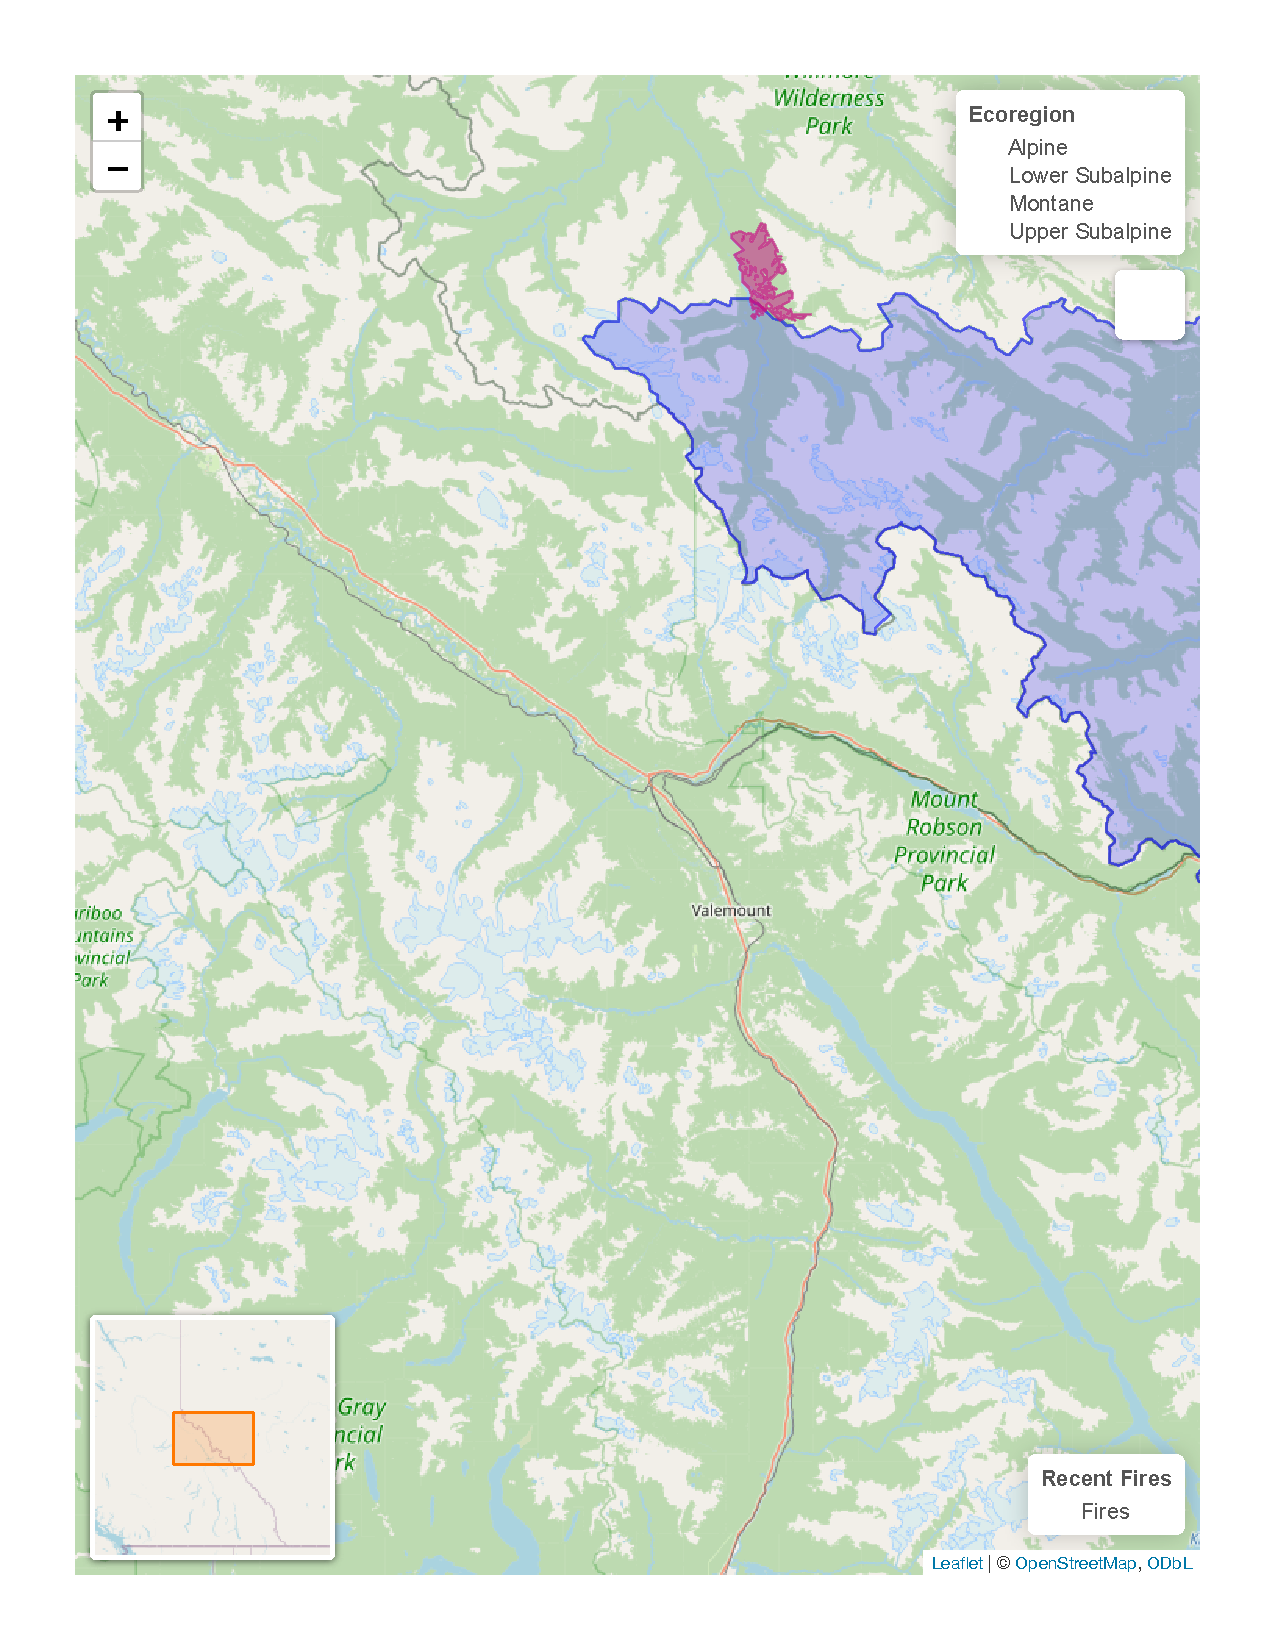
\includegraphics[keepaspectratio]{janp_files/figure-pdf/fig-aru-monitoring-locations-1.pdf}}

}

\caption{\label{fig-aru-monitoring-locations}Locations from Jasper
National Park ARU EI Monitoring Program.}

\end{figure}%

\begin{Shaded}
\begin{Highlighting}[]
\FunctionTok{datatable}\NormalTok{(janp\_locs\_table, }
          \AttributeTok{options =} \FunctionTok{list}\NormalTok{(}
            \AttributeTok{searching =} \ConstantTok{TRUE}\NormalTok{,  }
            \AttributeTok{paging =} \ConstantTok{TRUE}\NormalTok{,    }
            \AttributeTok{pageLength =} \DecValTok{10}   
\NormalTok{          )) }\SpecialCharTok{|\textgreater{}}
  \FunctionTok{formatStyle}\NormalTok{(}\AttributeTok{columns =} \FunctionTok{colnames}\NormalTok{(janp\_locs\_table), }
              \AttributeTok{backgroundColor =} \FunctionTok{styleEqual}\NormalTok{(}\FunctionTok{c}\NormalTok{(}\StringTok{"NA"}\NormalTok{), }\StringTok{"lightgray"}\NormalTok{))  }
\end{Highlighting}
\end{Shaded}

\begin{table}

\caption{\label{tbl-loc-summary}Locations surveyed across years. Ones
indicated a deployment in that year for that location.}

\centering{

\pandocbounded{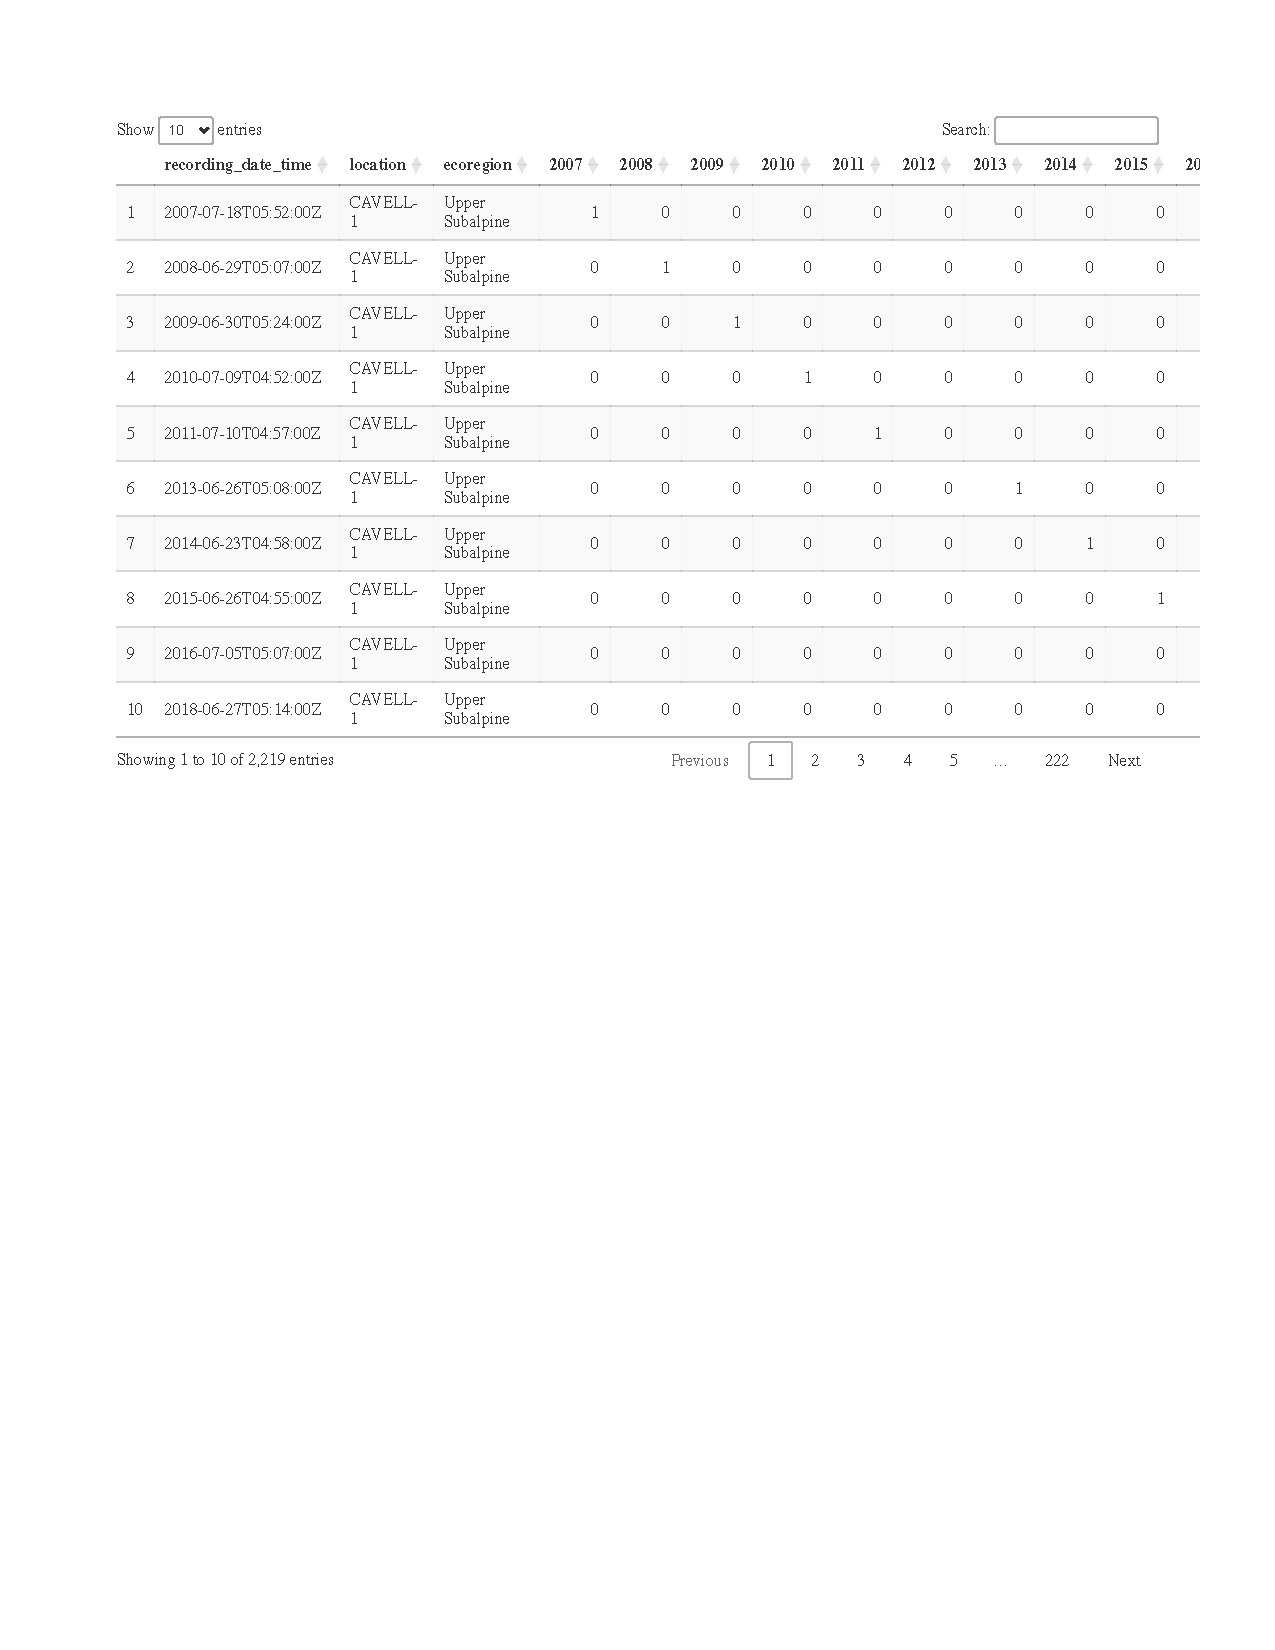
\includegraphics[keepaspectratio]{janp_files/figure-pdf/tbl-loc-summary-1.pdf}}

}

\end{table}%

\subsection{Habitat and survey
variables}\label{habitat-and-survey-variables}

We used the existing Vegetation Resource Inventory (VRI) derived from
2020 orthophoto imagery, before the 2022 Chetamon and 2024 Jasper
Wildfire to describe habitat conditions. We extracted variables
describing dominant land cover (including conifer, broadleaf, shrub,
herbaceous, and exposed soil classes), forest structure (canopy height,
age), and understory characteristics (shrub height, crown closure). To
account for the severe habitat alteration caused by the 2024 Jasper
Wildfire, we manually reclassified the land cover variable for all sites
on the TEKARRA and VALLEY5 transects as ``Burned'' for the 2025 data.
This classification replaced the pre-fire VRI categories (e.g., conifer,
shrub) in the analysis.

\subsection{Weather variables}\label{weather-variables}

To examine the influence of weather on species richness and abundance,
we fit a negative binomial generalized linear model (glm.nb()) with
richness as the response and temperature, sky (clear, overcast,
scattered), wind, Julian day, and hour as predictors. Model dispersion,
calculated as the ratio of residual deviance to residual degrees of
freedom, was 1.02, indicating minor overdispersion and suggesting an
adequate fit. Julian day (β = --0.014, p \textless{} 0.001) and hour (β
= --0.024, p = 0.002) were significantly negatively associated with
richness, while temperature, wind, and sky type showed weak or
non-significant effects. Although temperature and wind were not
significant in this model, they were retained in subsequent analyses due
to their known ecological influence on bat activity and detection
probability. The model residual deviance was 1527.5 on 1494 degrees of
freedom, with an AIC of 7684.5 and an estimated dispersion parameter (θ)
of 40.77 (SE = 8.59).

\subsection{Data management, processing and quality
control}\label{data-management-processing-and-quality-control}

Recordings were clipped and organized to only include the 10-minute
count. Before adopting WildTrax in 2021, processing analysts excluded
the initial 20 seconds to 1.5 minutes of recordings to reduce human
impact on detection probability, then logged the first detection time
per species. Recordings are now uploaded as clean 10-minute files with
the voice note and observer notes removed. In WildTrax, individuals were
counted by users scanning both the spectrogram and listening to the
audio output (MacPhail et al. (2026)). Tags were then drawn to encompass
the signal within the methods indicated in each project (see
Table~\ref{tbl-transcriptions}). Transcribers also had site photos
available to optimize their species identification by having habitat
context while processing.

To ensure comparability across the 18-year dataset, we harmonized the
abundance metrics derived from the differing transcription protocols
prior to analysis. For legacy data collected between 2012 and 2020 using
the 3-minute interval method, we calculated abundance as the maximum
count observed in any single time bin rather than summing across bins.
This conservative approach prevents the double-counting of individuals
that sing continuously throughout the recording. Conversely, for data
processed or re-transcribed using the modern 1SPT protocol (time of
first detection of each unique individual of each species; 2007--2011
and 2021--2025), abundance was defined as the total count of unique
individuals detected over the full 10-minute duration. Specifically, in
WildTrax maximum count of individuals was used (i.e.~AMRO1, AMRO2, AMRO3
max of 3 represents 3 individuals total).

\begin{Shaded}
\begin{Highlighting}[]
\NormalTok{transcription\_table }\OtherTok{\textless{}{-}} \FunctionTok{tibble}\NormalTok{(}
  \AttributeTok{Years =} \FunctionTok{c}\NormalTok{(}\StringTok{"2007{-}2020"}\NormalTok{, }\StringTok{"2021{-}2022"}\NormalTok{, }\StringTok{"2023{-}2025"}\NormalTok{, }\StringTok{"2007{-}2011"}\NormalTok{),}
  \StringTok{\textasciigrave{}}\AttributeTok{Transcription Method}\StringTok{\textasciigrave{}} \OtherTok{=} \FunctionTok{c}\NormalTok{(}
    \StringTok{"0{-}3.33, 3.33{-}6.66, 6.66{-}10 min"}\NormalTok{,}
    \StringTok{"1 SPT {-} Species per task or recording (Every new individual is tagged within the 10 minute recording)."}\NormalTok{,}
    \StringTok{"1 SPT {-} Species per task or recording (Every new individual is tagged within the 10 minute recording)."}\NormalTok{,}
    \StringTok{"1 SPT {-} Species per task or recording (Every new individual is tagged within the 10 minute recording). Re{-}transcription."}
\NormalTok{  ),}
  \StringTok{\textasciigrave{}}\AttributeTok{Bin Method}\StringTok{\textasciigrave{}} \OtherTok{=} \FunctionTok{c}\NormalTok{(}
    \StringTok{"Abundance re{-}starts for each 3.33{-}minute bin"}\NormalTok{,}
    \StringTok{"Time of first detection over 10 minute period"}\NormalTok{,}
    \StringTok{"Time of first detection over 10 minute period"}\NormalTok{,}
    \StringTok{"Time of first detection over 10 minute period. Re{-}transcription."}
\NormalTok{  ),}
  \StringTok{\textasciigrave{}}\AttributeTok{Method Details}\StringTok{\textasciigrave{}} \OtherTok{=} \FunctionTok{c}\NormalTok{(}
    \StringTok{"No cap on abundance; abundance re{-}starts for each bin, no total abundance for the 10{-}min recording"}\NormalTok{,}
    \StringTok{"Time of first detection over 10 minute period"}\NormalTok{,}
    \StringTok{"Time of first detection over 10 minute period"}\NormalTok{,}
    \StringTok{"Time of first detection over 10 minute period. Re{-}transcription."}
\NormalTok{  ),}
  \StringTok{\textasciigrave{}}\AttributeTok{Max \# of Individuals}\StringTok{\textasciigrave{}} \OtherTok{=} \FunctionTok{c}\NormalTok{(}
    \StringTok{"No cap"}\NormalTok{,}
    \StringTok{"Maximum of 3 individuals per 10{-}minute recording"}\NormalTok{,}
    \StringTok{"No cap"}\NormalTok{,}
    \StringTok{"No cap. Re{-}transcription."}
\NormalTok{  )}
\NormalTok{)}

\NormalTok{transcription\_table}
\DocumentationTok{\#\# \# A tibble: 4 x 5}
\DocumentationTok{\#\#   Years     \textasciigrave{}Transcription Method\textasciigrave{}                 \textasciigrave{}Bin Method\textasciigrave{} \textasciigrave{}Method Details\textasciigrave{}}
\DocumentationTok{\#\#   \textless{}chr\textgreater{}     \textless{}chr\textgreater{}                                  \textless{}chr\textgreater{}        \textless{}chr\textgreater{}           }
\DocumentationTok{\#\# 1 2007{-}2020 0{-}3.33, 3.33{-}6.66, 6.66{-}10 min         Abundance r\textasciitilde{} No cap on abund\textasciitilde{}}
\DocumentationTok{\#\# 2 2021{-}2022 1 SPT {-} Species per task or recording\textasciitilde{} Time of fir\textasciitilde{} Time of first d\textasciitilde{}}
\DocumentationTok{\#\# 3 2023{-}2025 1 SPT {-} Species per task or recording\textasciitilde{} Time of fir\textasciitilde{} Time of first d\textasciitilde{}}
\DocumentationTok{\#\# 4 2007{-}2011 1 SPT {-} Species per task or recording\textasciitilde{} Time of fir\textasciitilde{} Time of first d\textasciitilde{}}
\DocumentationTok{\#\# \# i 1 more variable: \textasciigrave{}Max \# of Individuals\textasciigrave{} \textless{}chr\textgreater{}}

\CommentTok{\# Render the datatable}
\FunctionTok{datatable}\NormalTok{(transcription\_table, }
          \AttributeTok{options =} \FunctionTok{list}\NormalTok{(}
            \AttributeTok{searching =} \ConstantTok{TRUE}\NormalTok{,  }
            \AttributeTok{paging =} \ConstantTok{TRUE}\NormalTok{,    }
            \AttributeTok{pageLength =} \DecValTok{10}   
\NormalTok{          )) }\SpecialCharTok{|\textgreater{}}
  \FunctionTok{formatStyle}\NormalTok{(}\AttributeTok{columns =} \FunctionTok{colnames}\NormalTok{(transcription\_table), }
              \AttributeTok{backgroundColor =} \FunctionTok{styleEqual}\NormalTok{(}\FunctionTok{c}\NormalTok{(}\StringTok{"NA"}\NormalTok{), }\StringTok{"lightgray"}\NormalTok{))  }
\end{Highlighting}
\end{Shaded}

\begin{table}

\caption{\label{tbl-transcriptions}Transcription methods by year
(2007--2025). Historical data (2007--2020) are undergoing
re-transcription to align with the standardized protocol used from 2021
onwards.}

\centering{

\pandocbounded{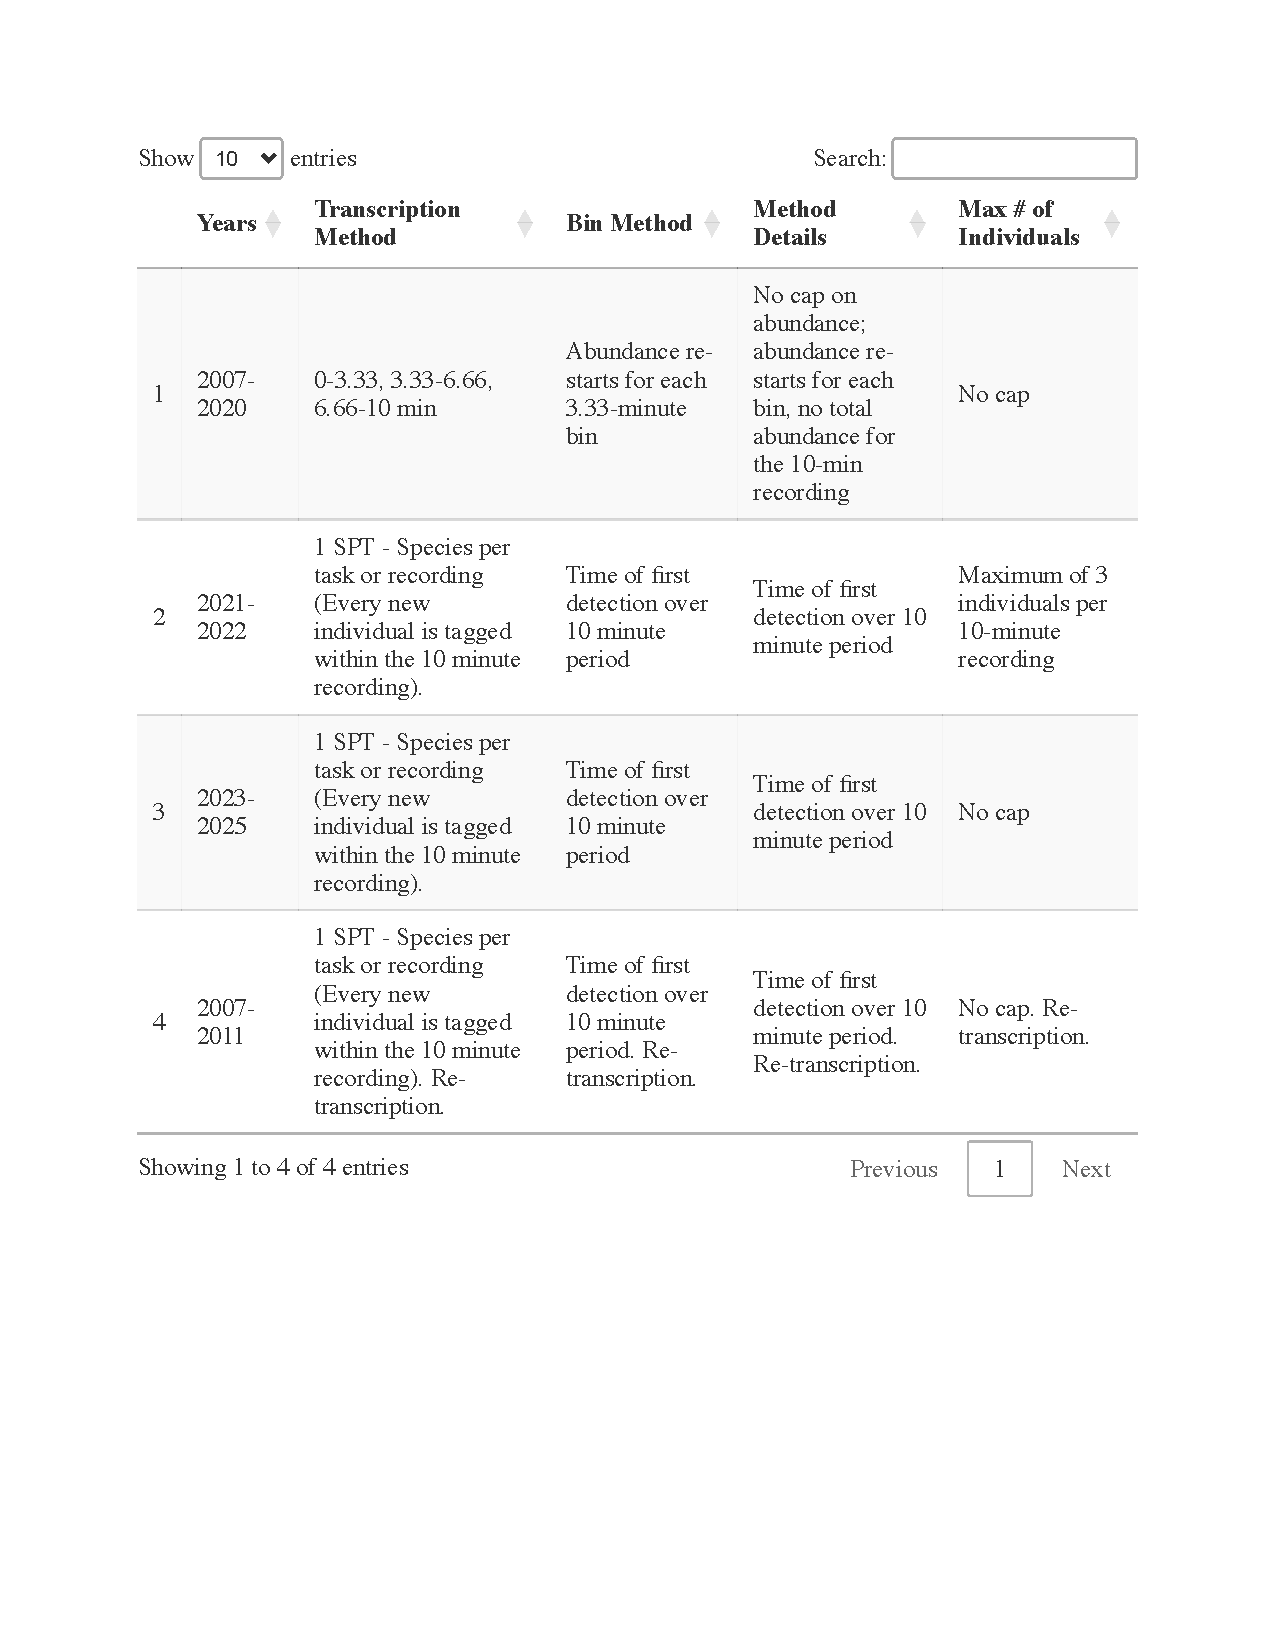
\includegraphics[keepaspectratio]{janp_files/figure-pdf/tbl-transcriptions-1.pdf}}

}

\end{table}%

\begin{figure}

\centering{

\pandocbounded{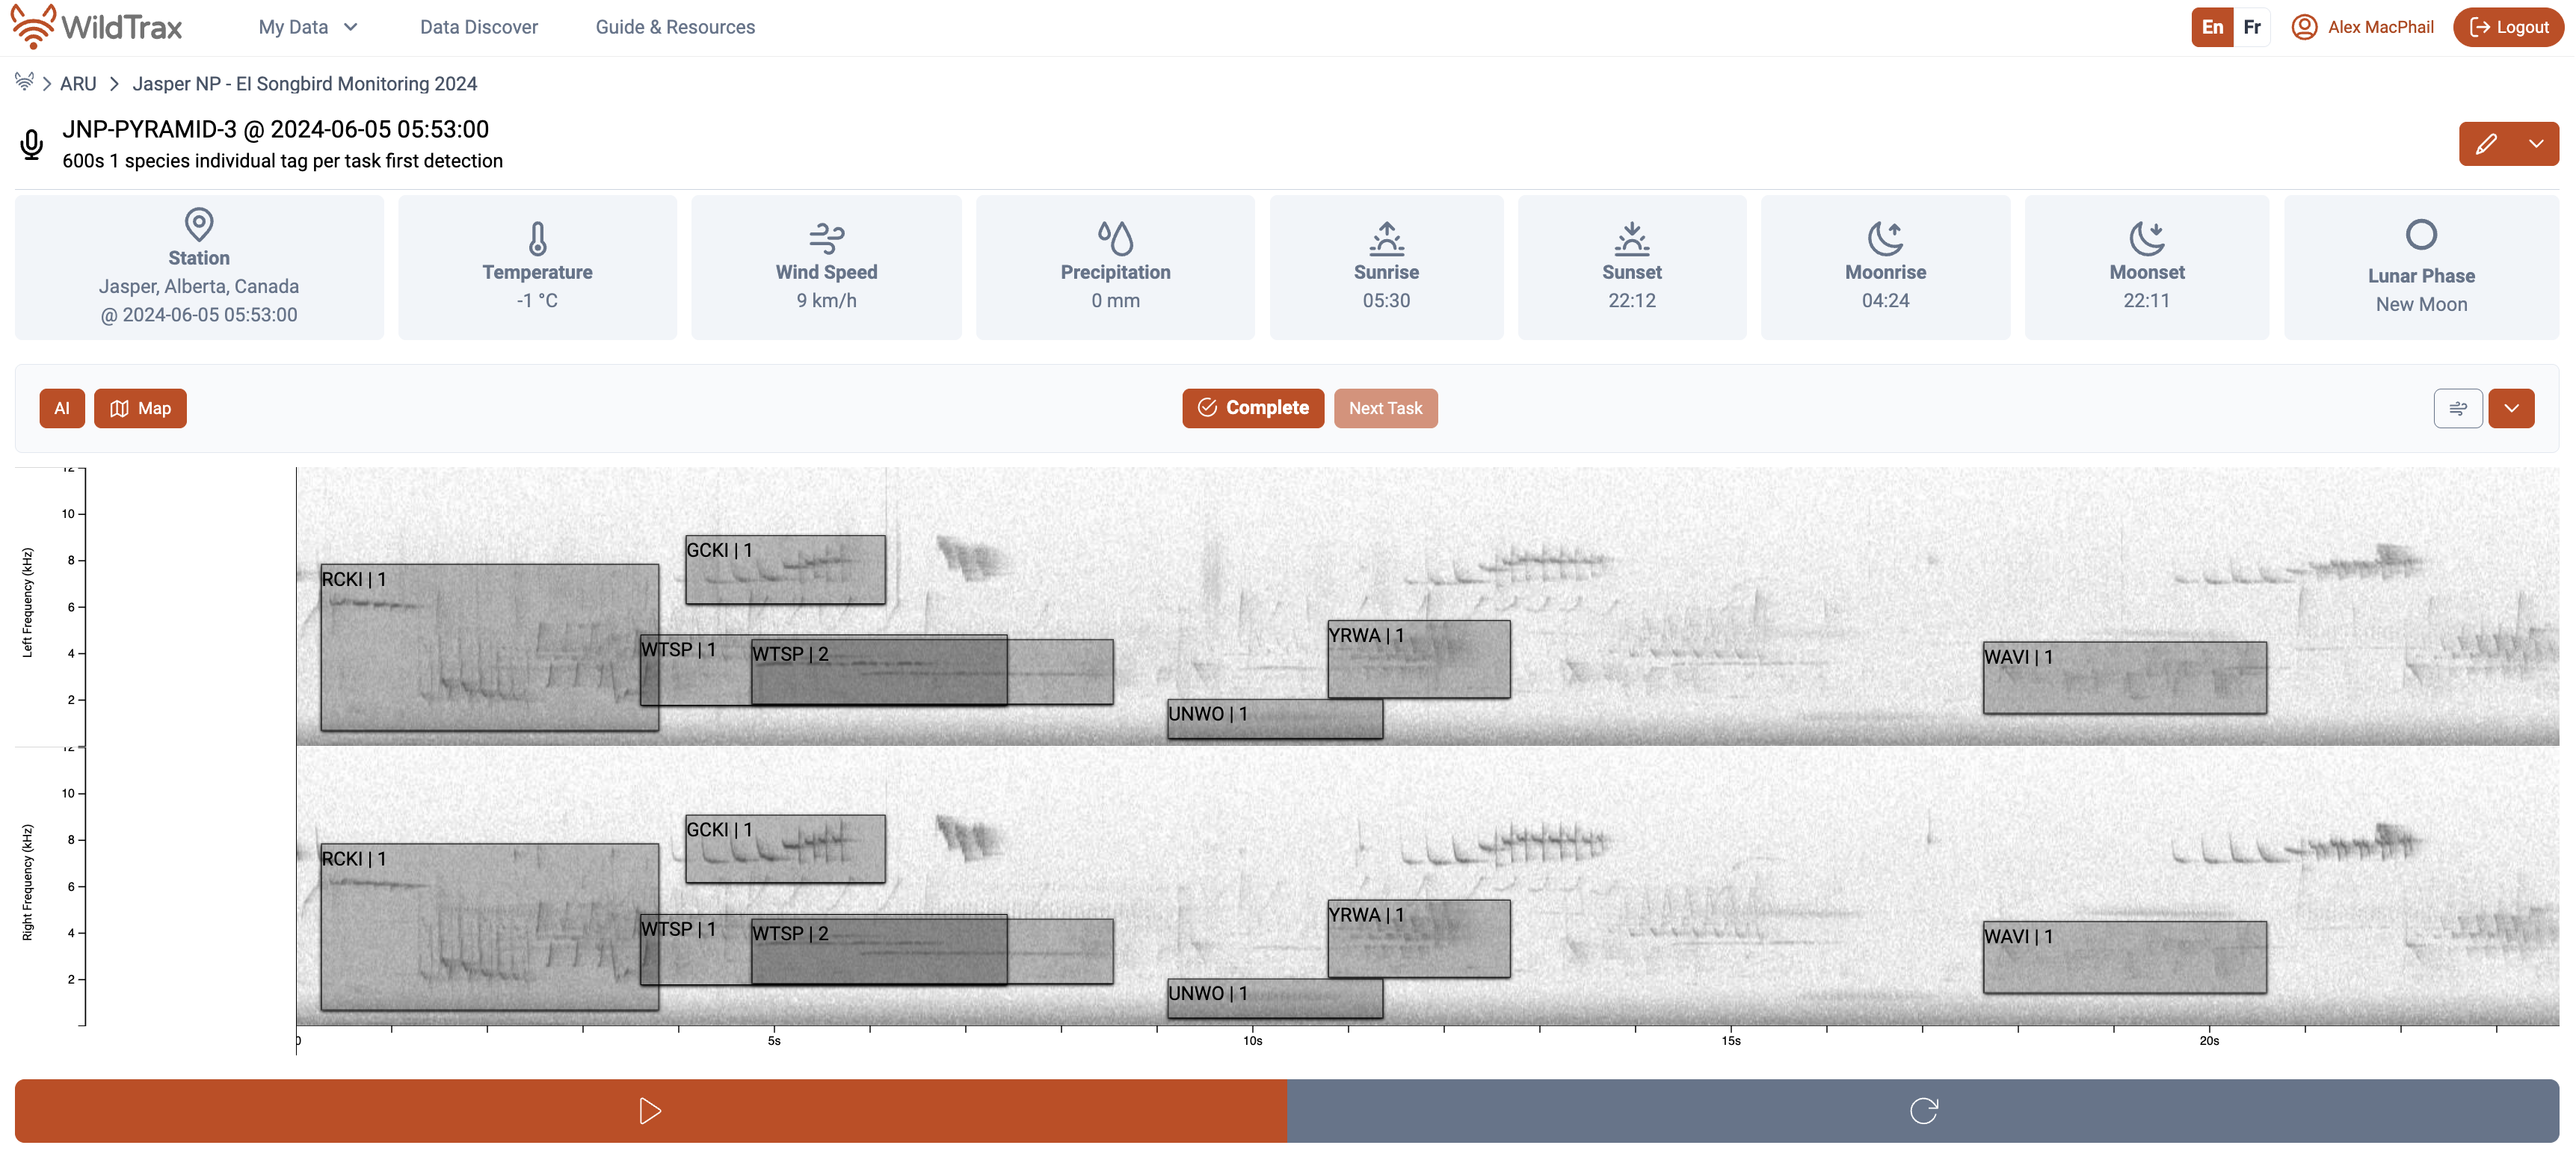
\includegraphics[keepaspectratio]{assets/acousticprocessing.png}}

}

\caption{\label{fig-acousticprocessing}WildTrax Acoustic Processing
Interface (Version 2)}

\end{figure}%

\pandocbounded{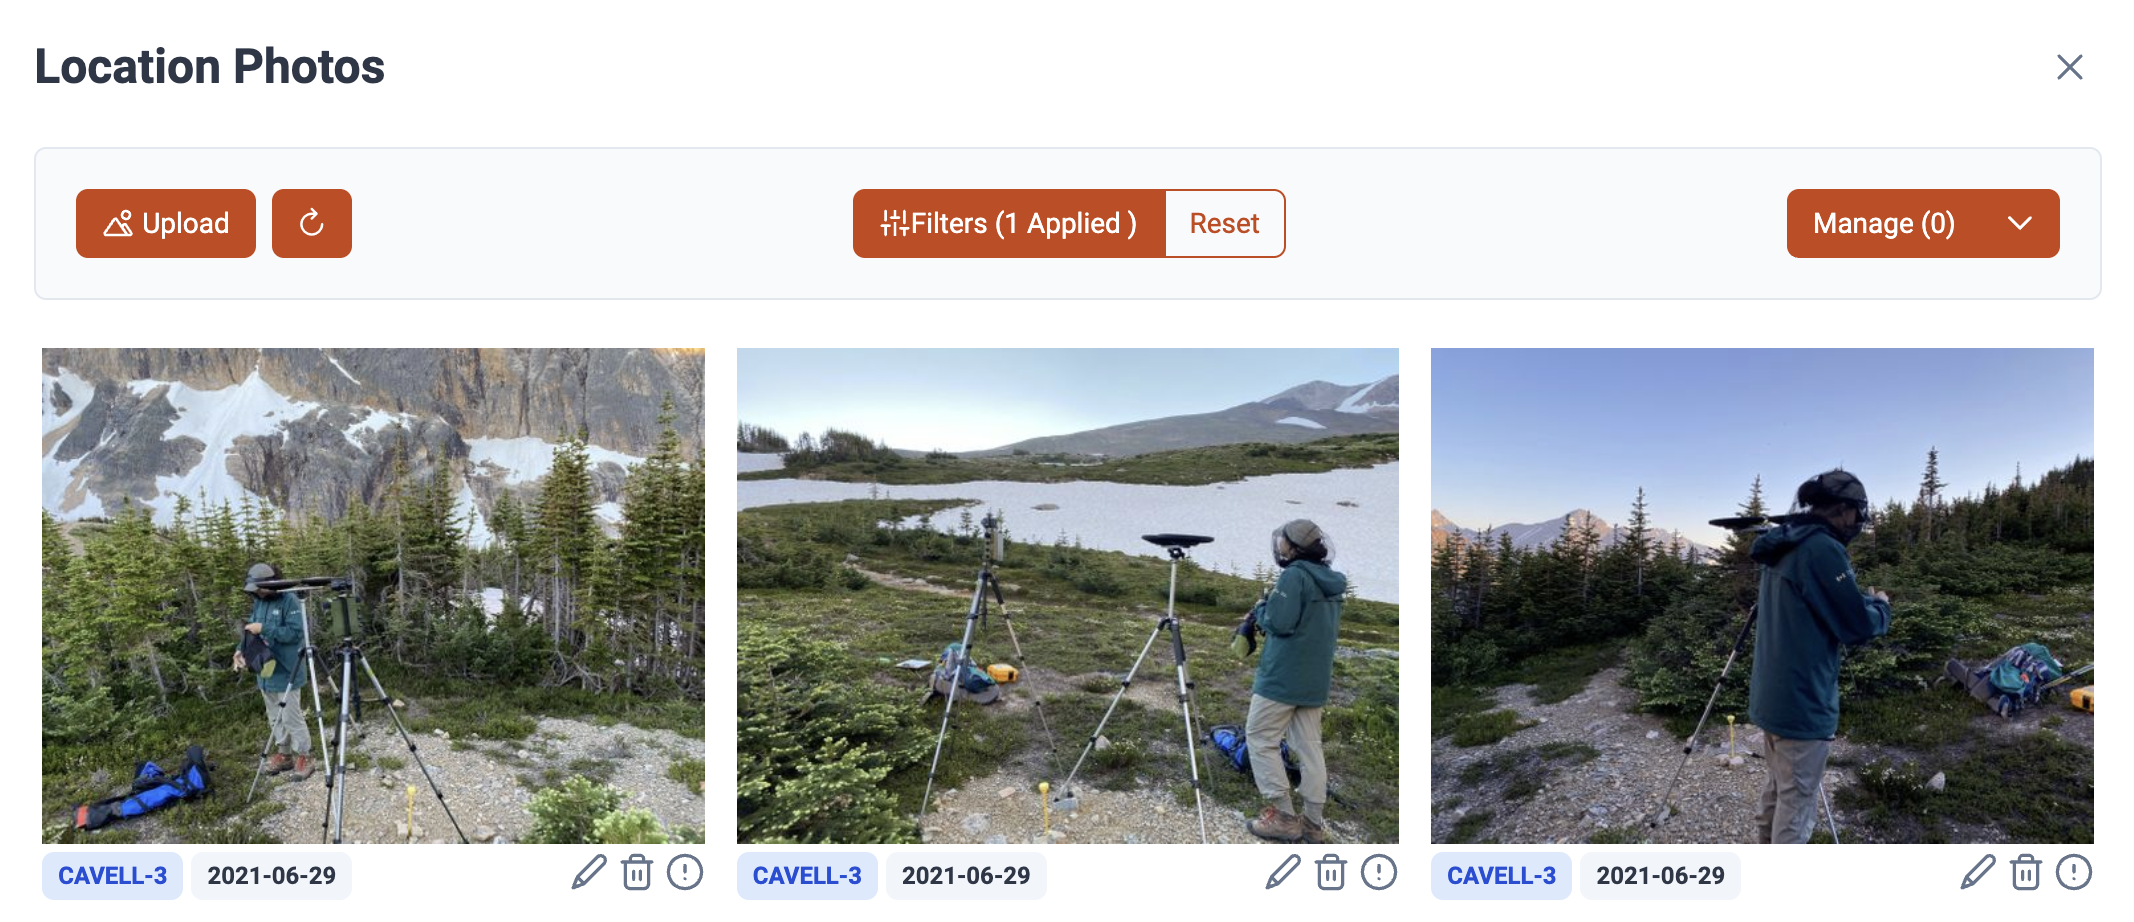
\includegraphics[keepaspectratio]{assets/locationphotos.png}}
We also evaluated the performance of the HawkEars and BirdNET
classifiers on the acoustic recordings (\textbf{?@fig-classifiers}).

\subsection{Analytical methods}\label{analytical-methods}

\begin{tcolorbox}[enhanced jigsaw, toptitle=1mm, title=\textcolor{quarto-callout-note-color}{\faInfo}\hspace{0.5em}{Note}, colback=white, colbacktitle=quarto-callout-note-color!10!white, opacitybacktitle=0.6, breakable, rightrule=.15mm, coltitle=black, toprule=.15mm, titlerule=0mm, left=2mm, bottomtitle=1mm, bottomrule=.15mm, arc=.35mm, leftrule=.75mm, opacityback=0, colframe=quarto-callout-note-color-frame]

For the purpose of these analyses, abundance was defined as the count of
individuals detected during point counts, rather than as a density x
area relationship. All analyses took place in R 4.5.2 `{[}Not{]} Part in
a Rumble'.

\end{tcolorbox}

Our analysis proceeded in the following steps. We:

\begin{itemize}
\tightlist
\item
  Assessed if the new forest sites were effective controls for
  fire-affected sites;
\item
  Evaluated consistency in species identification and abundance
  estimates between transcription methods and observers;
\item
  Selected species and grouped species by guild for trend analysis;
\end{itemize}

\subsubsection{Location correlation}\label{sec-location-correction}

To inform our subsequent modeling choices, we first evaluated the bird
survey data for spatial autocorrelation (e.g., survey points close to
one another exhibit similar bird counts). To test for this, we
calculated a total abundance index for each location and year by summing
the maximum number of individuals detected, representing the minimum
number of individuals known to be present. Because survey points were
typically spaced 300 m apart, we defined spatial neighbor relationships
using a 1-nearest-neighbor approach (\emph{k} = 1) based on great-circle
distances. We derived spatial coordinates from geographic point data,
excluding non-finite values to ensure valid estimation. Using the
\texttt{knearneigh()} and \texttt{knn2nb()} functions in R, we
constructed a spatial weights matrix with row-standardized weights to
reflect immediate adjacency between points. We assessed global spatial
autocorrelation in total abundance using Moran's \emph{I} under a
randomization assumption. This statistic evaluates whether the landscape
is spatially structured---specifically, whether nearby locations tend to
have similar abundance values more often than expected by chance. To
determine if this dependence was driven by localized clustering, we
further calculated Local Indicators of Spatial Association (LISA) using
local Moran's \emph{I}. This allowed for the identification of potential
high--high, low--low, and spatial outlier patterns, with statistical
significance evaluated at \emph{α} = 0.05. While global Moran's \emph{I}
indicated significant positive spatial autocorrelation across the study
area, local Moran's \emph{I} revealed no statistically significant
clusters. This pattern suggests that similarities in bird counts among
nearby survey locations were spread broadly rather than concentrated in
distinct hotspots, consistent with spatial dependence arising from
gradual, landscape‑scale ecological processes rather than localized
aggregations. Therefore, we proceeded by treating the locations as
spatially independent.

\subsubsection{Control site comparisons}\label{control-site-comparisons}

The 2024 Jasper Wildfire severely burned two established acoustic
transects (VALLEY5 and TEKKARA). While only one-third of true montane
(valley-bottom) forest has burnt since 2023, two of three transects were
severely burned. To continue to monitor bird communities in unburned
forest, we added two control transects in 2025 in the true montane
(COTTONWOOD and MUSHROOM), and we plan to continue to monitor both the
burned and control transects.

To assess whether the new transects were appropriate controls for
montane transects, we evaluated how similar their species assemblages
were to those observed at existing true montane transects over the past
three years, excluding the TEKARRA5 and VALLEY5 transects post-fire
because these were expected to diverge substantially due to fire
severity. Specifically, we compared species detections from the
COTTONWOOD and MUSHROOM transects to the distribution of detections
across all other true montane points to quantify compositional
similarity and departure from the true montane baseline.
Representativeness of control transects was assessed using a
multivariate dispersion analysis (PERMDISP) based on Bray--Curtis
dissimilarity, with distances of control transects to the true montane
centroid compared against the distribution of distances among
established true montane transects. Statistical significance of
differences in dispersion was evaluated using a permutation test with
999 iterations.

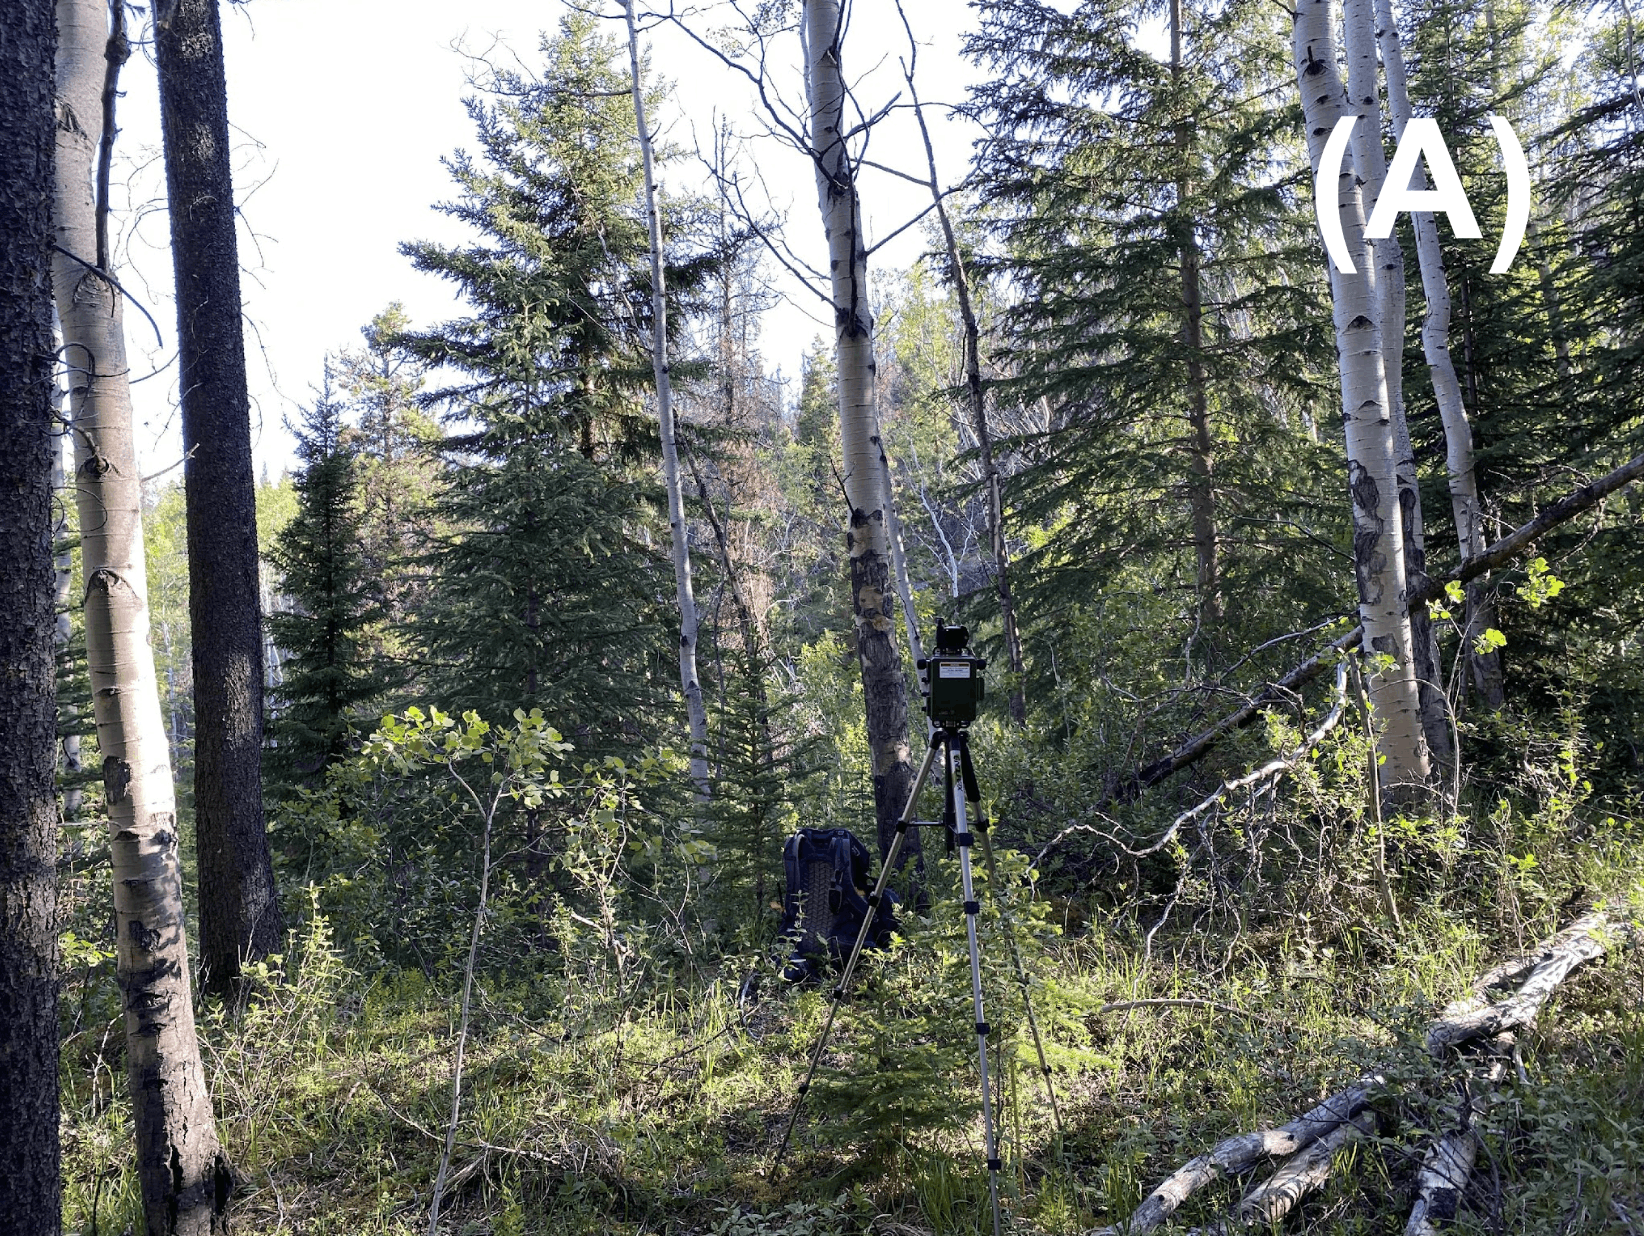
\includegraphics[width=0.48\linewidth,height=\textheight,keepaspectratio]{assets/tekarra9-2024.png}
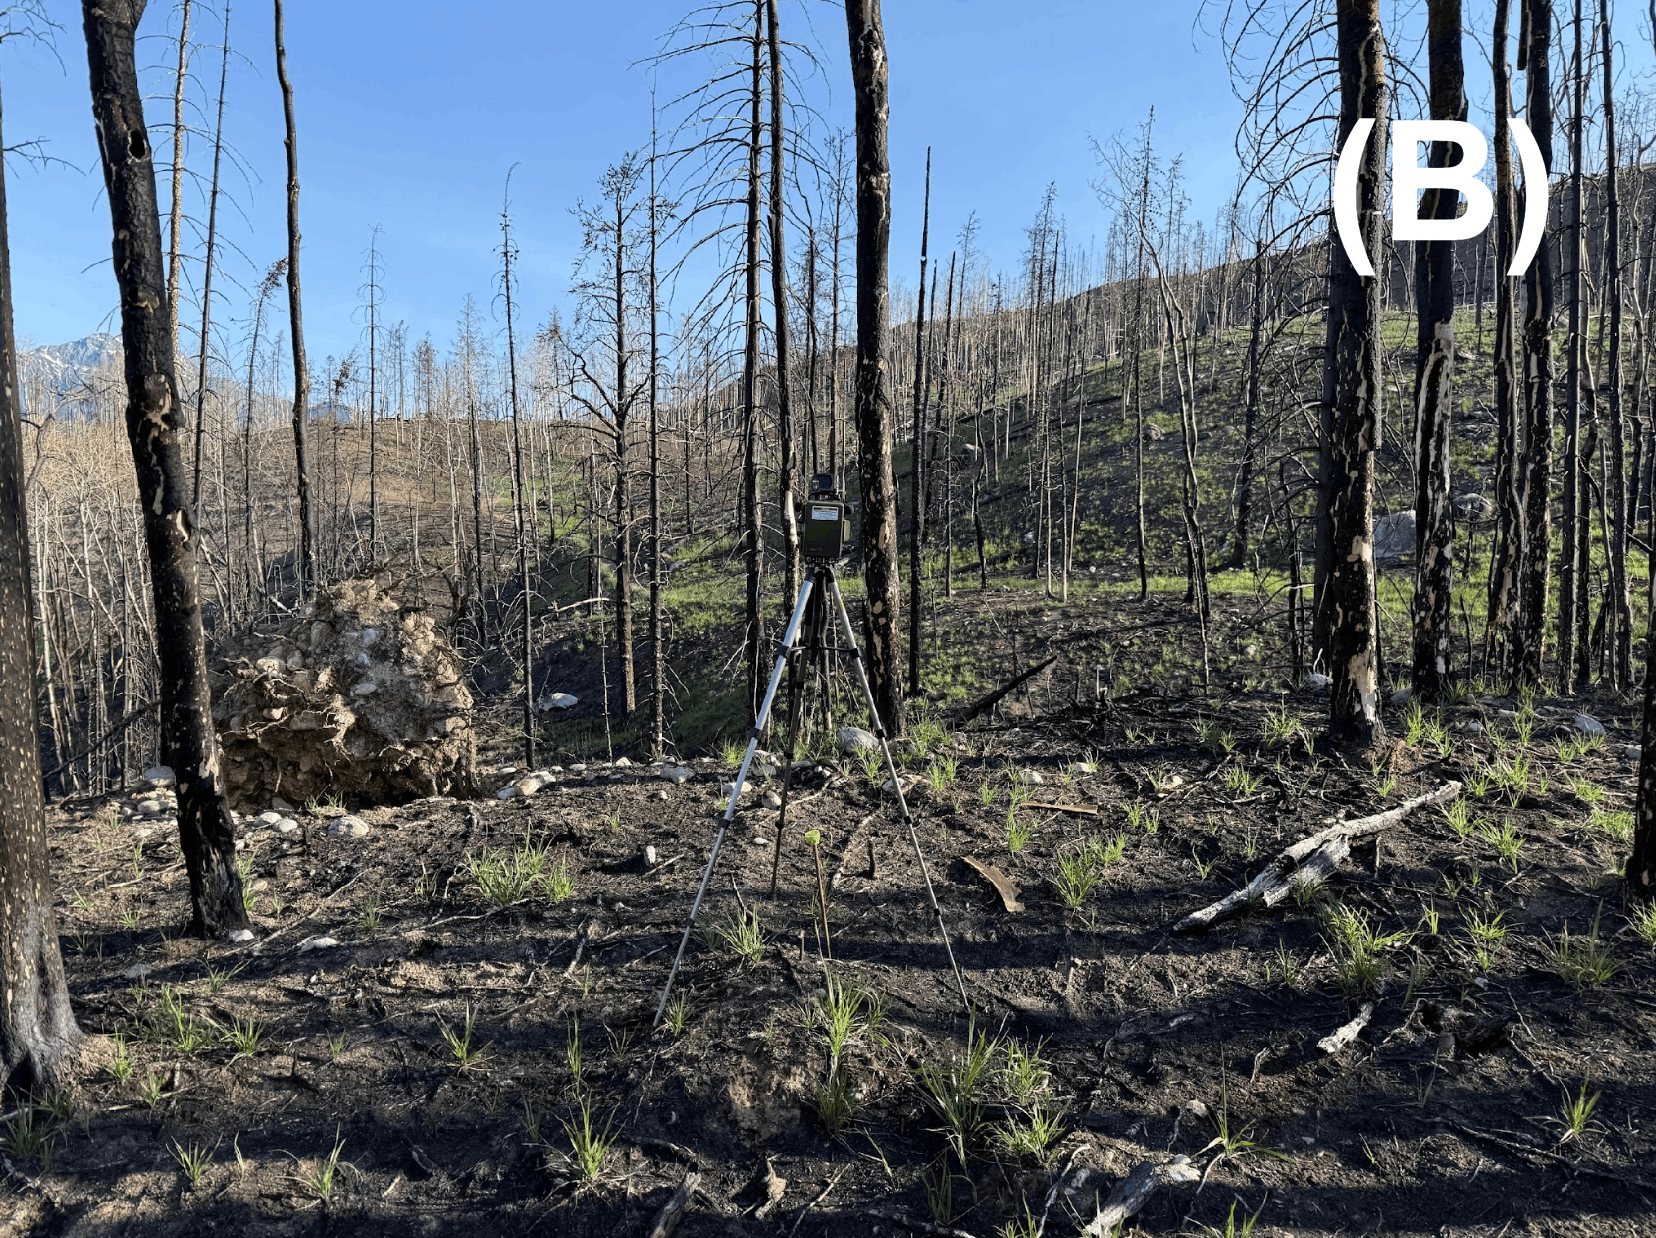
\includegraphics[width=0.48\linewidth,height=\textheight,keepaspectratio]{assets/tekarra9-2025.png}

Tekarra 9 site photos views from 2024 (A) pre-fire, and 2025 (B)
post-fire.

\subsubsection{Transcription observer
comparisons}\label{transcription-observer-comparisons}

Transcription methods varied (Table~\ref{tbl-transcriptions}) over time.
Recordings from 2007 to 2020 were classified by a small number of repeat
observers (legacy), while subsequent data were classified by a random
selection from many observers (WildTrax). To evaluate consistency
between the legacy dataset and the modern WildTrax workflow, we analyzed
a subset of recordings processed using both approaches. This included
re-processed legacy recordings that 1) enabled total abundance estimates
and 2) used new observers in WildTrax, allowing for direct comparison of
individual observer performance between the legacy and modern protocols.
For each dual-processed recording, we derived the maximum count of
individuals per species identified by each specific observer. We used
two different metrics to verify data continuity.

First, to quantify consistency in abundance estimates, we calculated
pairwise Pearson correlations between all individual observers. These
relationships were visualized using a heatmap to identify any systematic
deviations in counting between legacy contractors and current WildTrax
observers. Figure~\ref{fig-pairwise} indicates that there is general
consistency in abundance counts, but not high reliability between
observers \hl{(e.g., some observers are more generous with counts than
others) indicating there may be a bias - OR BECAUSE METHOD CHANGED -
e.g., re-start between bins, cap on counts.}

Second, to evaluate consistency in species detection (composition), we
binarized the data to presence/absence and calculated Bray--Curtis
dissimilarities between individual observers. We then applied
hierarchical clustering to these dissimilarity scores to verify that the
transition to WildTrax did not introduce observer-specific biases in
species identification or community composition. Figure 4 shows that
most observers agree on species, and there doesn't appear to be a
systematic bias during the transition to WildTrax. If the transition
introduced a major bias, we would see two distinct large branches with
one containing all legacy contractors and one containing all WildTrax
observers. Data using both types of transcription observer method were
grouped for analysis, however when available for a given year, the
modern WildTrax workflow results were used because they included total
abundance estimates (Table~\ref{tbl-transcriptions}).

\begin{figure}

\centering{

\pandocbounded{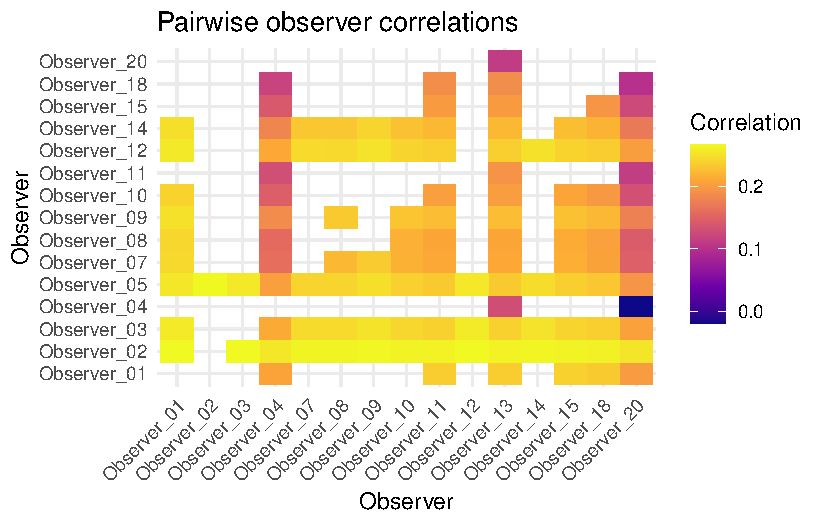
\includegraphics[keepaspectratio]{janp_files/figure-pdf/fig-pairwise-1.pdf}}

}

\caption{\label{fig-pairwise}Heatmap visualizes how consistently
different observers recorded abundance estimates. Yellow indicates
strong positive correlation (high reliability between observers),
orange/red indicates weak positive correlation (general consistency) and
dark purple indicates a diversion in counts while white appears where
there are no overlapping observations to compare.}

\end{figure}%

\subsubsection{Selection of species and guilds for trend
analysis}\label{selection-of-species-and-guilds-for-trend-analysis}

\begin{Shaded}
\begin{Highlighting}[]
\NormalTok{species\_select }\OtherTok{\textless{}{-}}\NormalTok{ janp\_main }\SpecialCharTok{|\textgreater{}}
  \FunctionTok{mutate}\NormalTok{(}\AttributeTok{species\_code =} \FunctionTok{case\_when}\NormalTok{(species\_code }\SpecialCharTok{==} \StringTok{"VESP"} \SpecialCharTok{\textasciitilde{}} \StringTok{"FOSP"}\NormalTok{, }\ConstantTok{TRUE} \SpecialCharTok{\textasciitilde{}}\NormalTok{ species\_code)) }\SpecialCharTok{|\textgreater{}}
  \FunctionTok{filter}\NormalTok{(}\SpecialCharTok{!}\NormalTok{(species\_code }\SpecialCharTok{\%in\%} \FunctionTok{c}\NormalTok{(}\StringTok{"NONE"}\NormalTok{,}\StringTok{"DOGG"}\NormalTok{,}\StringTok{"HOMA"}\NormalTok{,}\StringTok{"UROPAR"}\NormalTok{,}\StringTok{"HORS"}\NormalTok{,}\StringTok{"VIRA"}\NormalTok{))) }\SpecialCharTok{|\textgreater{}}
  \FunctionTok{filter}\NormalTok{(}\SpecialCharTok{!}\NormalTok{(}\FunctionTok{grepl}\NormalTok{(}\StringTok{\textquotesingle{}\^{}Unidentified\textquotesingle{}}\NormalTok{,species\_common\_name))) }\SpecialCharTok{|\textgreater{}}
  \FunctionTok{group\_by}\NormalTok{(species\_code) }\SpecialCharTok{|\textgreater{}}
  \FunctionTok{tally}\NormalTok{() }\SpecialCharTok{|\textgreater{}}
  \FunctionTok{inner\_join}\NormalTok{(}\FunctionTok{wt\_get\_species}\NormalTok{() }\SpecialCharTok{|\textgreater{}}\NormalTok{ dplyr}\SpecialCharTok{::}\FunctionTok{select}\NormalTok{(species\_code, species\_common\_name, species\_order, species\_class) }\SpecialCharTok{|\textgreater{}} \FunctionTok{distinct}\NormalTok{())}
\end{Highlighting}
\end{Shaded}

\begin{verbatim}
Joining with `by = join_by(species_code)`
\end{verbatim}

The monitoring program dataset produced detections for 143 species of
birds and 6 species of mammals (American Pika, Elk, Hoary Marmot, Red
Squirrel, Columbian Ground Squirrel and White-tailed Deer). Following
recommendations in the literature Prowse et al. (2021), we focused on
native terrestrial species for which: (a) Jasper National Park is their
breeding range; and (b) the total count across all point count sites
exceeded 20 individuals (see Table~\ref{tbl-guilds}).

To assess trends in species' abundances and interpret community-level
ecological responses, we assigned species to guilds. Guilds are groups
of species that respond in similar ways to environmental changes as a
result of similar uses of the environment (Doser et al. (2021)).
Directional trends in abundant species (e.g., Yellow-rumped warbler
(\emph{Setophaga coronata}, YRWA)) can strongly influence the trend of
the guilds of which these species are members. Given this limitation,
trend analyses of ecological guilds often warrant further examination of
common patterns of change among species within the guild. For example,
if we find large variation in abundance trends across an ecoregion but
not across bird guilds, this may suggest a consistent effect on the
entire bird community (Doser et al. (2021)), which can determine if
management should target a whole community, specific guilds or
individual species. If all or many species within a guild show similar
trends in relative abundance, then factors affecting the guild-related
life history attributes deserve attention. Pacifici et al. (2014)
recommend using bird guilds in post-hoc assessment. Each species was
categorized within guilds and a species may be included in multiple
guilds. Species were assigned to guilds using the
\href{https://birdsna.org}{Birds of North America},
\href{https://esajournals.onlinelibrary.wiley.com/doi/10.1890/13-1917.1}{Elton
Traits Database} and bird guidebooks. To examine responses by different
guild types we assigned birds by Elton trait (e.g., invertebrate,
plant/seed, omnivore), dietary guild (e.g., aerial insectivore, bark
forager), and habitat guild (e.g., wetland, forest generalist, late
successional forest) (Table~\ref{tbl-guilds}).

\subsubsection{Ecoregion community composition
analysis}\label{ecoregion-community-composition-analysis}

To characterize bird community composition, we first aggregated
species-level observations into a species-by-location matrix, populated
with the maximum count of each species at each location. Survey points
were then classified into two primary ecoregions: alpine and montane
(high elevation forest). For the purpose of this analysis, the montane
category served as a broad aggregate, grouping the upper subalpine,
lower subalpine, and montane ecoregions into a single unit that refers
to high elevation habitat below treeline. We quantified the variation in
community composition explained by these two ecoregions using Redundancy
Analysis (RDA) in the vegan package (Oksanen et al. (2025)) and
visualized species--ecoregion relationships with ordination plots (C.
Radhakrishna Rao (1964)). Finally, to test for statistical differences
in composition between the Alpine and Montane groups, we performed a
permutational multivariate analysis of variance (PERMANOVA; Anderson
(2001)). This test was conducted on Bray--Curtis dissimilarities using
999 permutations under a reduced model.

\subsubsection{Functional and community-level
diversity}\label{functional-and-community-level-diversity}

To evaluate community-level ecological responses, we examined temporal
changes in functional diversity, species richness, and community
structure. First, we quantified functional diversity using Rao's
\emph{Q} (C. R. Rao (1982); Laliberté and Legendre (2010)), calculated
via the \texttt{dbFD()} function in the \texttt{FD} package (Laliberté,
Legendre, and Shipley (2014)). This metric estimates the average
difference in functional traits between any two random individuals in
the community. We also calculated species richness (number of unique
species per location per year) and Shannon's diversity index, which
integrates richness and evenness to describe community structure. These
metrics were modeled through time using linear, mixed-effects, and
segmented regression models to detect both gradual and threshold-type
changes. Results were summarized graphically by ecoregion and functional
guild to highlight spatial variation in diversity trajectories. We also
calculated species richness (number of unique species per location per
year) and Shannon's diversity index, which integrates richness and
evenness to describe community structure. We assessed temporal changes
in Shannon diversity and species richness using a linear mixed-effects
model, with Shannon diversity and species count as the response
variable. Year was centered at the mean to estimate temporal trends, and
ecoregion (alpine vs.~forested) was included as a fixed effect to
account for differences between the two ecoregions. We included a random
intercept for each location and the model was fit using restricted
maximum likelihood (REML) with the \texttt{lmer()} function from the
\texttt{lme4} package.

\begin{table}

\caption{\label{tbl-guilds}Guilds}

\centering{

\pandocbounded{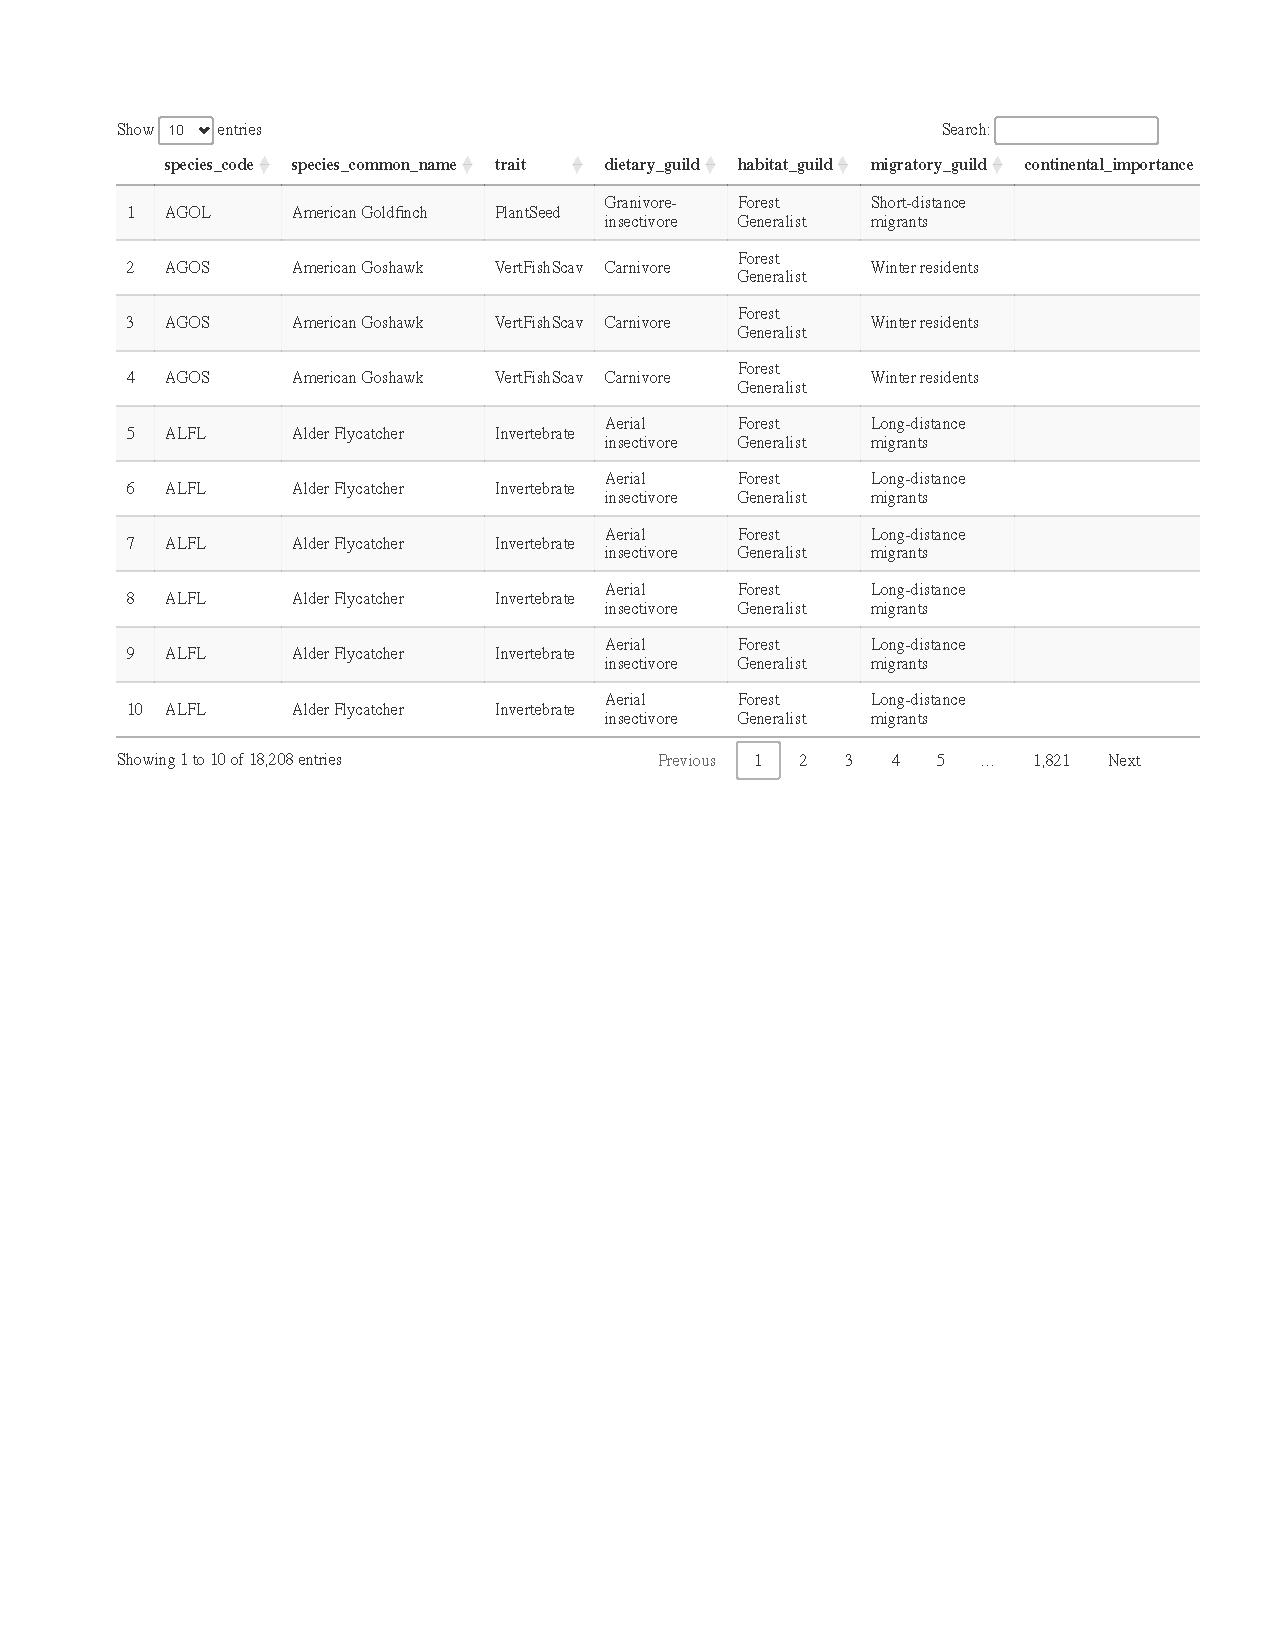
\includegraphics[keepaspectratio]{janp_files/figure-pdf/tbl-guilds-1.pdf}}

}

\end{table}%

\begin{Shaded}
\begin{Highlighting}[]
\NormalTok{shannon\_d }\OtherTok{\textless{}{-}}\NormalTok{ janp\_main }\SpecialCharTok{|\textgreater{}} 
  \FunctionTok{filter}\NormalTok{(}\SpecialCharTok{!}\FunctionTok{grepl}\NormalTok{(}\StringTok{\textquotesingle{}COTTONWOOD|MUSHROOM\textquotesingle{}}\NormalTok{, location)) }\SpecialCharTok{|\textgreater{}}
  \FunctionTok{mutate}\NormalTok{(}\AttributeTok{ecoregion =} \FunctionTok{case\_when}\NormalTok{(ecoregion }\SpecialCharTok{\%in\%} \FunctionTok{c}\NormalTok{(}\StringTok{"Alpine"}\NormalTok{) }\SpecialCharTok{\textasciitilde{}} \StringTok{"Alpine"}\NormalTok{,}
\NormalTok{                               ecoregion }\SpecialCharTok{\%in\%} \FunctionTok{c}\NormalTok{(}\StringTok{"Upper Subalpine"}\NormalTok{,}\StringTok{"Lower Subalpine"}\NormalTok{,}\StringTok{"Montane"}\NormalTok{) }\SpecialCharTok{\textasciitilde{}} \StringTok{"Montane"}\NormalTok{)) }\SpecialCharTok{|\textgreater{}}
  \FunctionTok{wt\_tidy\_species}\NormalTok{(}\AttributeTok{remove =} \FunctionTok{c}\NormalTok{(}\StringTok{"mammal"}\NormalTok{,}\StringTok{"amphibian"}\NormalTok{,}\StringTok{"abiotic"}\NormalTok{,}\StringTok{"insect"}\NormalTok{,}\StringTok{"unknown"}\NormalTok{), }\AttributeTok{zerofill =}\NormalTok{ F) }\SpecialCharTok{|\textgreater{}}
  \FunctionTok{inner\_join}\NormalTok{(}\FunctionTok{wt\_get\_species}\NormalTok{() }\SpecialCharTok{|\textgreater{}}\NormalTok{ dplyr}\SpecialCharTok{::}\FunctionTok{select}\NormalTok{(species\_code, species\_class, species\_order), }\AttributeTok{by =} \StringTok{"species\_code"}\NormalTok{) }\SpecialCharTok{|\textgreater{}}
\NormalTok{  dplyr}\SpecialCharTok{::}\FunctionTok{select}\NormalTok{(location, ecoregion, recording\_date\_time, species\_code, species\_common\_name, individual\_order, abundance) }\SpecialCharTok{|\textgreater{}}
  \FunctionTok{distinct}\NormalTok{() }\SpecialCharTok{|\textgreater{}}
  \FunctionTok{group\_by}\NormalTok{(location, ecoregion, recording\_date\_time, species\_code, species\_common\_name) }\SpecialCharTok{|\textgreater{}}
  \FunctionTok{summarise}\NormalTok{(}\AttributeTok{count =} \FunctionTok{max}\NormalTok{(individual\_order)) }\SpecialCharTok{|\textgreater{}}
  \FunctionTok{ungroup}\NormalTok{() }\SpecialCharTok{|\textgreater{}}
  \FunctionTok{pivot\_wider}\NormalTok{(}\AttributeTok{names\_from =}\NormalTok{ species\_code, }\AttributeTok{values\_from =}\NormalTok{ count, }\AttributeTok{values\_fill =} \DecValTok{0}\NormalTok{) }\SpecialCharTok{|\textgreater{}}
  \FunctionTok{pivot\_longer}\NormalTok{(}\AttributeTok{cols =} \SpecialCharTok{{-}}\NormalTok{(location}\SpecialCharTok{:}\NormalTok{species\_common\_name), }\AttributeTok{names\_to =} \StringTok{"species"}\NormalTok{, }\AttributeTok{values\_to =} \StringTok{"count"}\NormalTok{) }\SpecialCharTok{|\textgreater{}}
  \FunctionTok{group\_by}\NormalTok{(location, ecoregion, }\AttributeTok{year =} \FunctionTok{year}\NormalTok{(recording\_date\_time), species) }\SpecialCharTok{|\textgreater{}}
  \FunctionTok{summarise}\NormalTok{(}\AttributeTok{total\_count =} \FunctionTok{sum}\NormalTok{(count)) }\SpecialCharTok{|\textgreater{}}
  \FunctionTok{ungroup}\NormalTok{() }\SpecialCharTok{|\textgreater{}}
  \FunctionTok{group\_by}\NormalTok{(location, ecoregion, year) }\SpecialCharTok{|\textgreater{}}
  \FunctionTok{summarise}\NormalTok{(}\AttributeTok{shannon\_index =} \FunctionTok{diversity}\NormalTok{(total\_count, }\AttributeTok{index =} \StringTok{"shannon"}\NormalTok{)) }\SpecialCharTok{|\textgreater{}}
  \FunctionTok{ungroup}\NormalTok{() }\SpecialCharTok{|\textgreater{}}
  \FunctionTok{filter}\NormalTok{(}\SpecialCharTok{!}\NormalTok{(year }\SpecialCharTok{==} \DecValTok{2012} \SpecialCharTok{\&}\NormalTok{ ecoregion }\SpecialCharTok{==} \StringTok{"Montane"}\NormalTok{))}

\NormalTok{shannon\_d}\SpecialCharTok{$}\NormalTok{year\_c }\OtherTok{\textless{}{-}}\NormalTok{ shannon\_d}\SpecialCharTok{$}\NormalTok{year }\SpecialCharTok{{-}} \FunctionTok{mean}\NormalTok{(shannon\_d}\SpecialCharTok{$}\NormalTok{year)}
\NormalTok{shannon\_d}\SpecialCharTok{$}\NormalTok{ecoregion }\OtherTok{\textless{}{-}} \FunctionTok{factor}\NormalTok{(shannon\_d}\SpecialCharTok{$}\NormalTok{ecoregion, }\AttributeTok{levels =} \FunctionTok{c}\NormalTok{(}\StringTok{"Alpine"}\NormalTok{, }\StringTok{"Montane"}\NormalTok{))}
\NormalTok{shannon\_mod }\OtherTok{\textless{}{-}} \FunctionTok{lmer}\NormalTok{(shannon\_index }\SpecialCharTok{\textasciitilde{}}\NormalTok{ year\_c }\SpecialCharTok{+}\NormalTok{ ecoregion }\SpecialCharTok{+}\NormalTok{ (}\DecValTok{1}\SpecialCharTok{|}\NormalTok{location), }\AttributeTok{data =}\NormalTok{ shannon\_d)}
\FunctionTok{summary}\NormalTok{(shannon\_mod)}

\NormalTok{spp\_rich\_location }\OtherTok{\textless{}{-}}\NormalTok{ janp\_main }\SpecialCharTok{|\textgreater{}}
  \FunctionTok{filter}\NormalTok{(}\SpecialCharTok{!}\FunctionTok{grepl}\NormalTok{(}\StringTok{\textquotesingle{}COTTONWOOD|MUSHROOM\textquotesingle{}}\NormalTok{, location)) }\SpecialCharTok{|\textgreater{}}
  \FunctionTok{filter}\NormalTok{(data\_type }\SpecialCharTok{\%in\%} \FunctionTok{c}\NormalTok{(}\StringTok{"legacy"}\NormalTok{,}\StringTok{"single\_visit\_3\_max"}\NormalTok{,}\StringTok{"single\_visit\_0\_max"}\NormalTok{)) }\SpecialCharTok{|\textgreater{}}
  \FunctionTok{filter}\NormalTok{(}\SpecialCharTok{!}\NormalTok{(data\_type }\SpecialCharTok{==} \StringTok{"single\_visit\_0\_max"} \SpecialCharTok{\&}\NormalTok{ year }\SpecialCharTok{\textless{}} \DecValTok{2023}\NormalTok{)) }\SpecialCharTok{|\textgreater{}}
  \FunctionTok{wt\_tidy\_species}\NormalTok{(}\AttributeTok{remove =} \FunctionTok{c}\NormalTok{(}\StringTok{"mammal"}\NormalTok{,}\StringTok{"amphibian"}\NormalTok{,}\StringTok{"abiotic"}\NormalTok{,}\StringTok{"insect"}\NormalTok{,}\StringTok{"unknown"}\NormalTok{), }\AttributeTok{zerofill =}\NormalTok{ F) }\SpecialCharTok{|\textgreater{}}
\NormalTok{  dplyr}\SpecialCharTok{::}\FunctionTok{select}\NormalTok{(location, year, species\_code) }\SpecialCharTok{|\textgreater{}}
  \FunctionTok{distinct}\NormalTok{() }\SpecialCharTok{|\textgreater{}}
  \FunctionTok{group\_by}\NormalTok{(location, year) }\SpecialCharTok{|\textgreater{}}
  \FunctionTok{summarise}\NormalTok{(}\AttributeTok{species\_count =} \FunctionTok{n\_distinct}\NormalTok{(species\_code)) }\SpecialCharTok{|\textgreater{}}
  \FunctionTok{ungroup}\NormalTok{() }\SpecialCharTok{|\textgreater{}}
  \FunctionTok{inner\_join}\NormalTok{(locs\_summary, }\AttributeTok{by =} \FunctionTok{c}\NormalTok{(}\StringTok{"location"} \OtherTok{=} \StringTok{"Location"}\NormalTok{)) }\SpecialCharTok{|\textgreater{}}
  \FunctionTok{mutate}\NormalTok{(}\AttributeTok{ecoregion =} \FunctionTok{case\_when}\NormalTok{(ecoregion }\SpecialCharTok{\%in\%} \FunctionTok{c}\NormalTok{(}\StringTok{"Alpine"}\NormalTok{) }\SpecialCharTok{\textasciitilde{}} \StringTok{"Alpine"}\NormalTok{,}
\NormalTok{                               ecoregion }\SpecialCharTok{\%in\%} \FunctionTok{c}\NormalTok{(}\StringTok{"Upper Subalpine"}\NormalTok{,}\StringTok{"Lower Subalpine"}\NormalTok{,}\StringTok{"Montane"}\NormalTok{) }\SpecialCharTok{\textasciitilde{}} \StringTok{"Montane"}\NormalTok{)) }\SpecialCharTok{|\textgreater{}}
  \FunctionTok{filter}\NormalTok{(}\SpecialCharTok{!}\NormalTok{(year }\SpecialCharTok{==} \DecValTok{2012} \SpecialCharTok{\&}\NormalTok{ ecoregion }\SpecialCharTok{==} \StringTok{"Montane"}\NormalTok{))}

\NormalTok{spp\_rich\_location}\SpecialCharTok{$}\NormalTok{year\_c }\OtherTok{\textless{}{-}}\NormalTok{ spp\_rich\_location}\SpecialCharTok{$}\NormalTok{year }\SpecialCharTok{{-}} \FunctionTok{mean}\NormalTok{(spp\_rich\_location}\SpecialCharTok{$}\NormalTok{year)}
\NormalTok{spp\_rich\_location}\SpecialCharTok{$}\NormalTok{ecoregion }\OtherTok{\textless{}{-}} \FunctionTok{factor}\NormalTok{(spp\_rich\_location}\SpecialCharTok{$}\NormalTok{ecoregion, }\AttributeTok{levels =} \FunctionTok{c}\NormalTok{(}\StringTok{"Alpine"}\NormalTok{, }\StringTok{"Montane"}\NormalTok{))}
\NormalTok{spp\_rich\_mod }\OtherTok{\textless{}{-}} \FunctionTok{lmer}\NormalTok{(species\_count }\SpecialCharTok{\textasciitilde{}}\NormalTok{ year\_c }\SpecialCharTok{+}\NormalTok{ ecoregion }\SpecialCharTok{+}\NormalTok{ (}\DecValTok{1}\SpecialCharTok{|}\NormalTok{location), }\AttributeTok{data =}\NormalTok{ spp\_rich\_location)}
\FunctionTok{summary}\NormalTok{(spp\_rich\_mod)}
\end{Highlighting}
\end{Shaded}

\subsubsection{Trend analysis}\label{trend-analysis}

To quantify temporal changes in bird populations and community
composition from 2007 to 2025, we analyzed trends in species-specific
abundance, in montane and alpine assemblages separately, and grouping
species by functional guilds. Analyses were designed to separate
biological change from potential sampling and methodological effects,
ensuring that observed patterns represented genuine ecological
responses. This was achieved through a multi-step framework that (1)
evaluated (1) modeled detection probability and methodological
variability, (2) estimated detection-corrected abundance, and (3)
evaluated long-term directional trends and associated shifts in
functional and community-level diversity.

\paragraph{Location correlation}\label{location-correlation}

To inform modeling choices, we assessed spatial autocorrelation among
bird survey locations across years. We examined the spatial relationship
between survey points based on total species abundance per location and
year in order to determine whether spatial clustering or spatial
dependence exists in the species abundance data. Because survey points
were typically spaced 300 m apart, we defined spatial neighbor
relationships using a 1-nearest-neighbor approach (\emph{k} = 1) based
on great-circle distances. We derived spatial coordinates from
geographic point data, excluding non-finite values to ensure valid
estimation. Using the \texttt{knearneigh()} and \texttt{knn2nb()} in the
\texttt{spdep} package in R, we constructed a spatial weights matrix
with row-standardized weights to reflect immediate adjacency between
points.

We assessed global spatial autocorrelation in total abundance using
Moran's \emph{I} under a randomization assumption. This statistic
evaluates whether the landscape is spatially structured; whether nearby
locations tend to have similar abundance values more often than expected
by chance. To determine if this dependence was driven by localized
clustering, we further calculated Local Indicators of Spatial
Association (LISA) using local Moran's \emph{I}. This allowed for the
identification of potential high--high, low--low, and spatial outlier
patterns, with statistical significance evaluated at α = 0.05.

While global Moran's \emph{I} indicated significant positive spatial
autocorrelation across the study area, local Moran's \emph{I} revealed
no statistically significant clusters. This pattern suggests that
similarities in bird counts among nearby survey locations were spread
broadly rather than concentrated in distinct hotspots, consistent with
spatial dependence arising from gradual, landscape‑scale ecological
processes rather than localized aggregations. Therefore, we proceeded by
treating the locations as spatially independent.

\paragraph{Detection-corrected abundance
estimation}\label{detection-corrected-abundance-estimation}

Abundance was estimated using single-visit n-mixture abundance models
implemented in the \texttt{detect::svabu()} function (Sólymos, Lele, and
Bayne (2012)). This framework jointly models site-level abundance with
observation and detection probability from single-visit counts as
conditional likelihood estimates. The package and framework make it easy
for users to add and interpret observation and detection covariates
which supports logistical considerations for single-visit surveys. We
first stratified analyses by ecoregion (alpine vs.~forest), fitting
separate detection-abundance models given the assumption site
characteristics and ecological drivers are different in both ecoregions.
Expected abundance per site visit was modelled using the latent
abundance component (λ) specified as a function of interannual
variation, local observation covariates and detection covariates. For
the observation covariates, proportional landcover was measured within a
150-m buffer and classified into shrub, herbaceous cover, conifer cover,
bedrock and other. Canopy cover, and mean canopy height were computed as
observation-level predictors. Separate models were fitted using canopy
cover and height as detection covariates but models failed to converge
due to overdispersion and low sample size. Detectability was modelled
simultaneously using julian date, hour of day, temperature (degrees C)
and wind (km/h). Although we modeled for differences between observers,
and structural vegetation influences on detection probability (see Yip,
Knight, and Bayne (2025)), which included once again canopy height and
canopy cover at the point level, models failed to converge. Abundance
was modeled with a log link, and detection probability with a logit
link. Conditional maximum likelihood estimates were used, with model fit
assessed via log-likelihood and AIC with successful models below:

\begin{verbatim}
    log(λi​)=β0​+β1​yearc,i​+β2​shrubi​+β3​confi​+β4​avg_heighti​+β5​canopy_coveri​.
    
\end{verbatim}

where detection (or availability) probability was modeled, and,

\logit(pi)=α0+α1 temperaturei+α2 windi+α3 juliani+α4 houri.\logit(p\_i)
= \alpha\_0 + \alpha\_1,\text{temperature}\_i + \alpha\_2,\text{wind}\_i
+ \alpha\_3,\text{julian}\_i + \alpha\_4,\text{hour}\_i
.\logit(pi\hspace{0pt})=α0\hspace{0pt}+α1\hspace{0pt}temperaturei\hspace{0pt}+α2\hspace{0pt}windi\hspace{0pt}+α3\hspace{0pt}juliani\hspace{0pt}+α4\hspace{0pt}houri\hspace{0pt}.

was used to generate standardized, detection-corrected expected
abundances (λ) for each site visit, which were then averaged by year to
produce annual abundance indices. These indices were subsequently used
to evaluate temporal trends in species abundance.

\paragraph{Trend estimation}\label{trend-estimation}

Temporal trends were quantified using the Mann--Kendall test (Mann
(1945a); Hamed (2009)), which detects monotonic directional change, and
Sen's Slope (Pranab Kumar Sen (1968)) to estimate the magnitude of those
trends. Both tests were implemented via the \texttt{modifiedmk} package
(Hamed and Rao (1998)) and applied to the detection-corrected abundance
estimates (λ̂).Sen's slope provides an estimate of the median annual rate
of change in the abundance index over the time series. To express this
rate in a standardized and interpretable way, we converted Sen's slope
to a percent change per year by dividing the estimated slope by the mean
annual abundance index across the full time series and multiplying by
100. This metric represents the average proportional change in abundance
per year, relative to the long-term mean abundance of the species in
that ecoregion. Positive values indicate increasing abundance, while
negative values indicate declining abundance.

\section{Results}\label{results}

\begin{tcolorbox}[enhanced jigsaw, toptitle=1mm, title=\textcolor{quarto-callout-note-color}{\faInfo}\hspace{0.5em}{Note}, colback=white, colbacktitle=quarto-callout-note-color!10!white, opacitybacktitle=0.6, breakable, rightrule=.15mm, coltitle=black, toprule=.15mm, titlerule=0mm, left=2mm, bottomtitle=1mm, bottomrule=.15mm, arc=.35mm, leftrule=.75mm, opacityback=0, colframe=quarto-callout-note-color-frame]

Some of these analyses are still a work-in-progress. Check back soon for
updates and additional details.

\end{tcolorbox}

\subsection{Control site comparisons}\label{control-site-comparisons-1}

Multivariate dispersion differed significantly between control and
reference montane transects (PERMDISP; \emph{F} = 4.05, \emph{p} =
0.05). Although control transects exhibited a slightly higher median
distance (mean = 0.421), their distributions overlapped strongly with
those of the true montane reference transects (Mean = 0.415), and there
was no evidence of increased dispersion or outliers unique to
replacement sites (Figure X). This suggests that replacement transects
are not compositionally distinct from existing montane transects and
fall within the natural variability of montane bird communities already
sampled. Consequently, the addition of replacement sites is unlikely to
introduce systematic bias, supporting their use as valid representatives
of montane bird communities for pre- and post-fire comparisons.

\subsection{Ecoregion community composition
analysis}\label{ecoregion-community-composition-analysis-1}

Figure~\ref{fig-community} shows the relationship between species and
ecoregion. The PERMANOVA test was performed using Bray-Curtis
dissimilarity to assess whether community composition significantly
differed between ecoregion groups. The analysis revealed a significant
difference in community composition between alpine and montane groups.
The ecoregion grouping explained approximately 27.85\% of the variation
in community composition, while residual variation accounted for
72.15\%. These findings indicate a substantial divergence in species
composition between ecoregion groups and helps to justify subsequent
analyses looking at trend differences between these areas.

\begin{figure}

\centering{

\pandocbounded{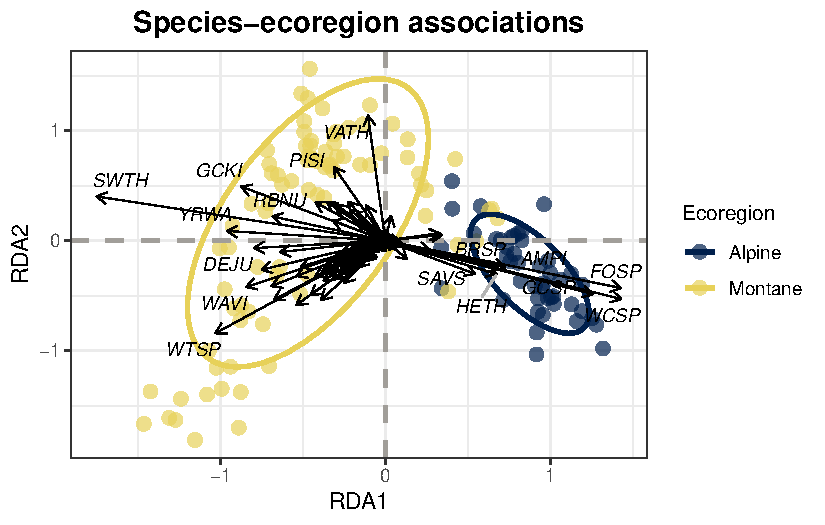
\includegraphics[keepaspectratio]{janp_files/figure-pdf/fig-community-1.pdf}}

}

\caption{\label{fig-community}}

\end{figure}%

\subsection{Functional and community-level
diversity}\label{functional-and-community-level-diversity-1}

Species richness per location is shown in Figure~\ref{fig-spp-rich-locs}
and Shannon's diversity over years is shown in Figure~\ref{fig-shannon}.
Shannon diversity increased slightly over time (β = 0.0063 per year, SE
= 0.0015, t = 4.20), after accounting for differences among locations
and ecoregions. Montane communities exhibited higher diversity than
Alpine (β = 0.28 ± 0.067, t = 4.15), and location-level variation
remained substantial (SD = 0.35). Rao's Q averaged between about 8.2 and
10.5 across survey locations, with a clear upward tendency over time
(Figure~\ref{fig-raos-q}). The non‑parametric Mann--Kendall test gave a
Kendall's τ of 0.32 (p ≈ 0.07), indicating a positive but marginally
non‑significant monotonic increase in functional diversity. A simple
linear regression of mean Rao's Q against year yielded a slope of 0.051
units per year (p ≈ 0.06), suggesting an upward trend that narrowly
misses the conventional 0.05 significance threshold. When comparing
models using an AIC-based approach, a segmented model clearly
outperformed both the linear model (ΔAIC = 2.97, weight = 0.18) and the
mixed-effects model (ΔAIC ≈ 11,883, weight ≈ 0), with the segmented
model having the lowest AIC (38.5, weight = 0.82). This supports the
presence of a breakpoint around 2009, suggesting that functional
diversity was relatively low and stable from 2007--2009, then increased
to more variable but generally higher values from 2010 onward. The
linear and mixed-effects models, while informative, were either slightly
less supported or poorly suited to capture this shift in the trend.

\begin{figure}

\centering{

\pandocbounded{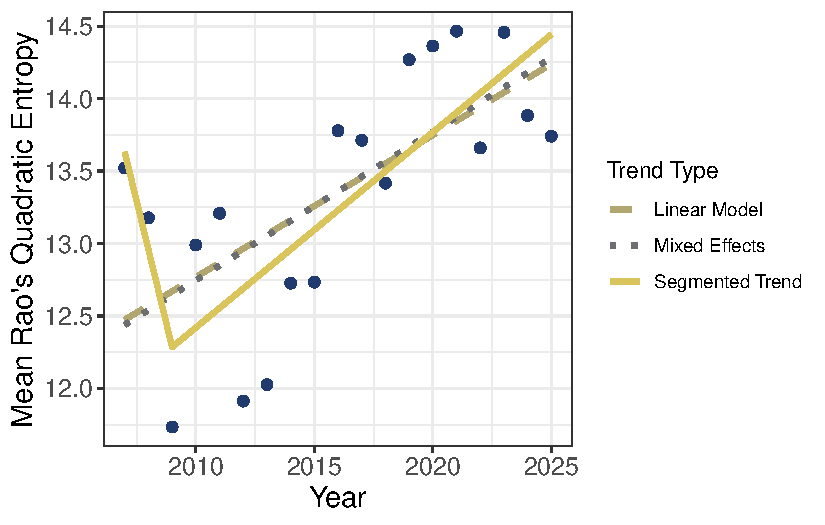
\includegraphics[keepaspectratio]{janp_files/figure-pdf/fig-raos-q-1.pdf}}

}

\caption{\label{fig-raos-q}Mean functional diversity (Rao's Q) over
time}

\end{figure}%

\begin{Shaded}
\begin{Highlighting}[]
\NormalTok{spp\_rich\_location }\SpecialCharTok{|\textgreater{}}
  \FunctionTok{ggplot}\NormalTok{(}\FunctionTok{aes}\NormalTok{(}\AttributeTok{x=}\FunctionTok{as.factor}\NormalTok{(year), }\AttributeTok{y=}\NormalTok{species\_count, }\AttributeTok{fill=}\NormalTok{year)) }\SpecialCharTok{+}
  \FunctionTok{geom\_boxplot}\NormalTok{() }\SpecialCharTok{+}
  \FunctionTok{geom\_point}\NormalTok{(}\AttributeTok{alpha =} \FloatTok{0.7}\NormalTok{, }\AttributeTok{colour =} \StringTok{"grey"}\NormalTok{) }\SpecialCharTok{+}
  \FunctionTok{geom\_smooth}\NormalTok{(}\AttributeTok{method =} \StringTok{"lm"}\NormalTok{) }\SpecialCharTok{+}
  \FunctionTok{theme\_bw}\NormalTok{() }\SpecialCharTok{+}
  \FunctionTok{facet\_wrap}\NormalTok{(}\SpecialCharTok{\textasciitilde{}}\NormalTok{ecoregion, }\AttributeTok{ncol =} \DecValTok{1}\NormalTok{) }\SpecialCharTok{+}
  \FunctionTok{scale\_fill\_viridis\_c}\NormalTok{(}\AttributeTok{option =} \StringTok{"cividis"}\NormalTok{) }\SpecialCharTok{+}
  \FunctionTok{xlab}\NormalTok{(}\StringTok{\textquotesingle{}Year\textquotesingle{}}\NormalTok{) }\SpecialCharTok{+} \FunctionTok{ylab}\NormalTok{(}\StringTok{\textquotesingle{}Species richness per location\textquotesingle{}}\NormalTok{) }\SpecialCharTok{+}
  \FunctionTok{guides}\NormalTok{(}\AttributeTok{fill =} \FunctionTok{guide\_legend}\NormalTok{(}\AttributeTok{title =} \StringTok{"Year"}\NormalTok{))}
\end{Highlighting}
\end{Shaded}

\begin{figure}[H]

\centering{

\pandocbounded{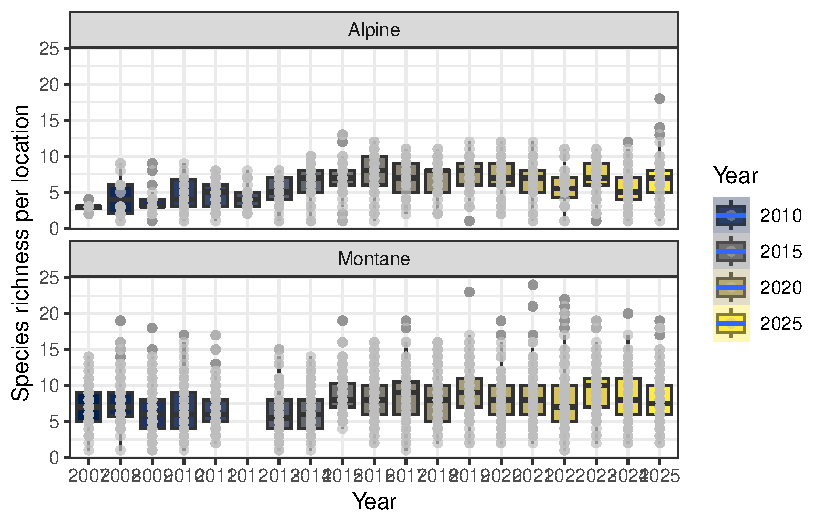
\includegraphics[keepaspectratio]{janp_files/figure-pdf/fig-spp-rich-locs-1.pdf}}

}

\caption{\label{fig-spp-rich-locs}Species richness by year. Data from
2012 were excluded for montane sites because those sites were not
sampled that year.}

\end{figure}%

\begin{Shaded}
\begin{Highlighting}[]
\NormalTok{shannon\_d }\SpecialCharTok{|\textgreater{}}
  \FunctionTok{ggplot}\NormalTok{(}\FunctionTok{aes}\NormalTok{(}\AttributeTok{x =} \FunctionTok{factor}\NormalTok{(year), }\AttributeTok{y =}\NormalTok{ shannon\_index, }\AttributeTok{fill =} \FunctionTok{factor}\NormalTok{(year))) }\SpecialCharTok{+}
  \FunctionTok{geom\_boxplot}\NormalTok{() }\SpecialCharTok{+}
  \FunctionTok{geom\_point}\NormalTok{(}\AttributeTok{alpha =} \FloatTok{0.6}\NormalTok{, }\AttributeTok{colour =} \StringTok{"grey"}\NormalTok{) }\SpecialCharTok{+}
  \FunctionTok{labs}\NormalTok{(}\AttributeTok{x =} \StringTok{"Year"}\NormalTok{,}
       \AttributeTok{y =} \StringTok{"Shannon diversity index per location"}\NormalTok{) }\SpecialCharTok{+}
  \FunctionTok{theme\_bw}\NormalTok{() }\SpecialCharTok{+}
  \FunctionTok{guides}\NormalTok{(}\AttributeTok{fill =} \FunctionTok{guide\_legend}\NormalTok{(}\AttributeTok{title =} \StringTok{"Year"}\NormalTok{)) }\SpecialCharTok{+}
  \FunctionTok{scale\_fill\_viridis\_d}\NormalTok{(}\AttributeTok{alpha =} \FloatTok{0.8}\NormalTok{, }\AttributeTok{option =} \StringTok{"cividis"}\NormalTok{) }\SpecialCharTok{+}
  \FunctionTok{facet\_wrap}\NormalTok{(}\SpecialCharTok{\textasciitilde{}}\NormalTok{ecoregion, }\AttributeTok{ncol =} \DecValTok{1}\NormalTok{)}
\end{Highlighting}
\end{Shaded}

\begin{figure}[H]

\centering{

\pandocbounded{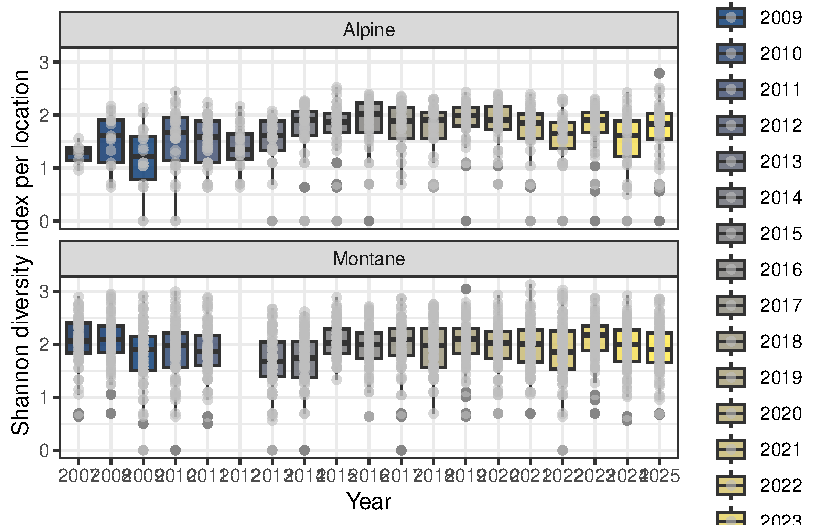
\includegraphics[keepaspectratio]{janp_files/figure-pdf/fig-shannon-1.pdf}}

}

\caption{\label{fig-shannon}Shannon diversity index across years. Data
from 2012 were excluded for montane sites because those sites were not
sampled that year.}

\end{figure}%

\subsection{Jasper 2024 fire effects}\label{jasper-2024-fire-effects}

The pre-fire and 1-year post-fire points occupy overlapping but shifted
regions indicating that the fire did not completely replace the
community but it reorganized species composition in a consistent
direction which is a classic disturbance-driven compositional shift and
not a collapse or a reset. In Figure~\ref{fig-after-fire}, the post-fire
ellipse is significantly shifted indicating greater variability among
sites after fire and more heterogeneous species assemblages. Species
vectors identified taxa contributing most strongly to these differences,
suggesting that the Jasper Wildfire altered species associations rather
than uniformly affecting overall abundance. Dark-eyed Junco (\emph{Junco
hyemalis}, DEJU) shows a strong directional association with post-fire
sites (they tolerate reduced canopy cover and more simplified forest
structure), while Swainson's Thrush (\emph{Catharus ustulatus}, SWTH),
Warbling Vireo (\emph{Vireo gilvus}, WAVI), and Tennessee Warbler
(\emph{Leiothlypis peregrina}, TEWA) were strongly associated with
pre-fire assemblages, and are generally associated with intact forest
canopy and vertical foliage structure. This indicates that structurally
complex forest conditions were an important component of bird community
composition prior to the Jasper Fire.

\begin{figure}

\centering{

\pandocbounded{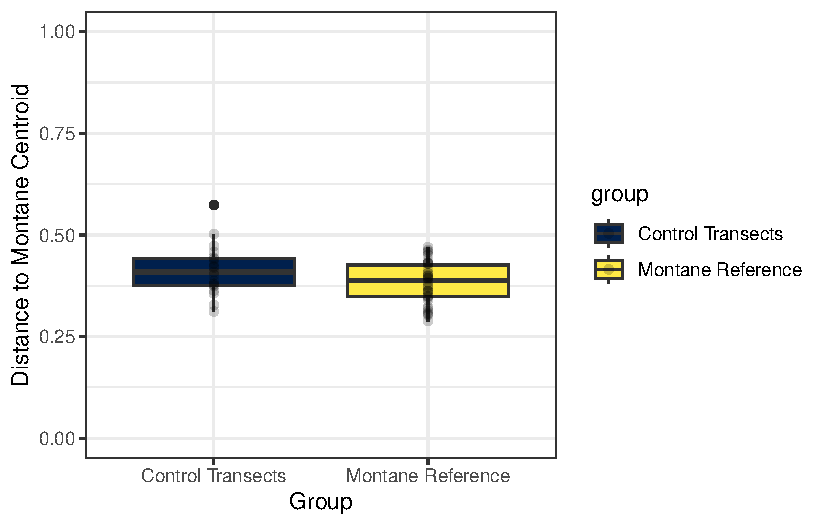
\includegraphics[keepaspectratio]{janp_files/figure-pdf/fig-control-transect-1.pdf}}

}

\caption{\label{fig-control-transect}Distances to the montane centroid
are similar (distributions overlap strongly) between the control and the
montane reference groups.}

\end{figure}%

\begin{figure}

\centering{

\pandocbounded{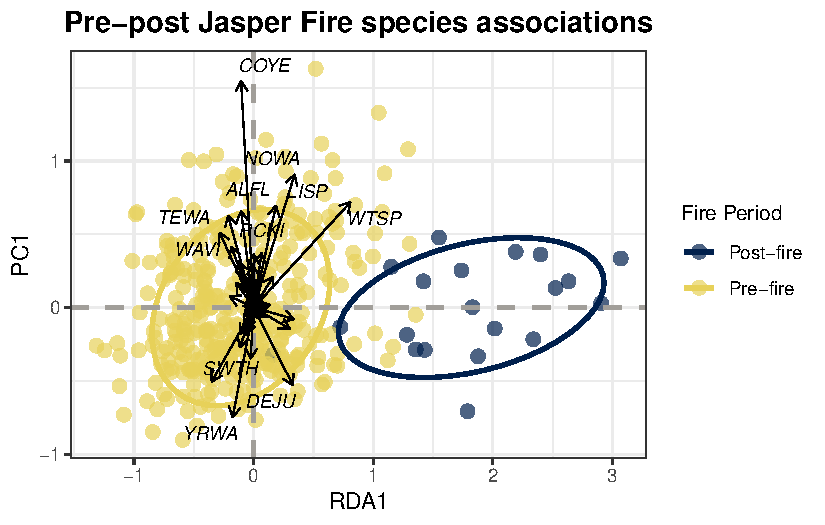
\includegraphics[keepaspectratio]{janp_files/figure-pdf/fig-after-fire-1.pdf}}

}

\caption{\label{fig-after-fire}Community matrix of species associations
before and after the Jasper 2024 fire on the VALLEY5 and TEKARRA
transects. Movement along RDA1 reflects the direction and magnitude of
fire-related change in species composition. PC1 captures residual
variation in species composition that is not explained by fire period
reflecting the background ecological variability among sites.}

\end{figure}%

\subsection{Trends}\label{trends}

\begin{table}

\caption{\label{tbl-trend}Summary of trend of species by ecoregion.}

\centering{

\pandocbounded{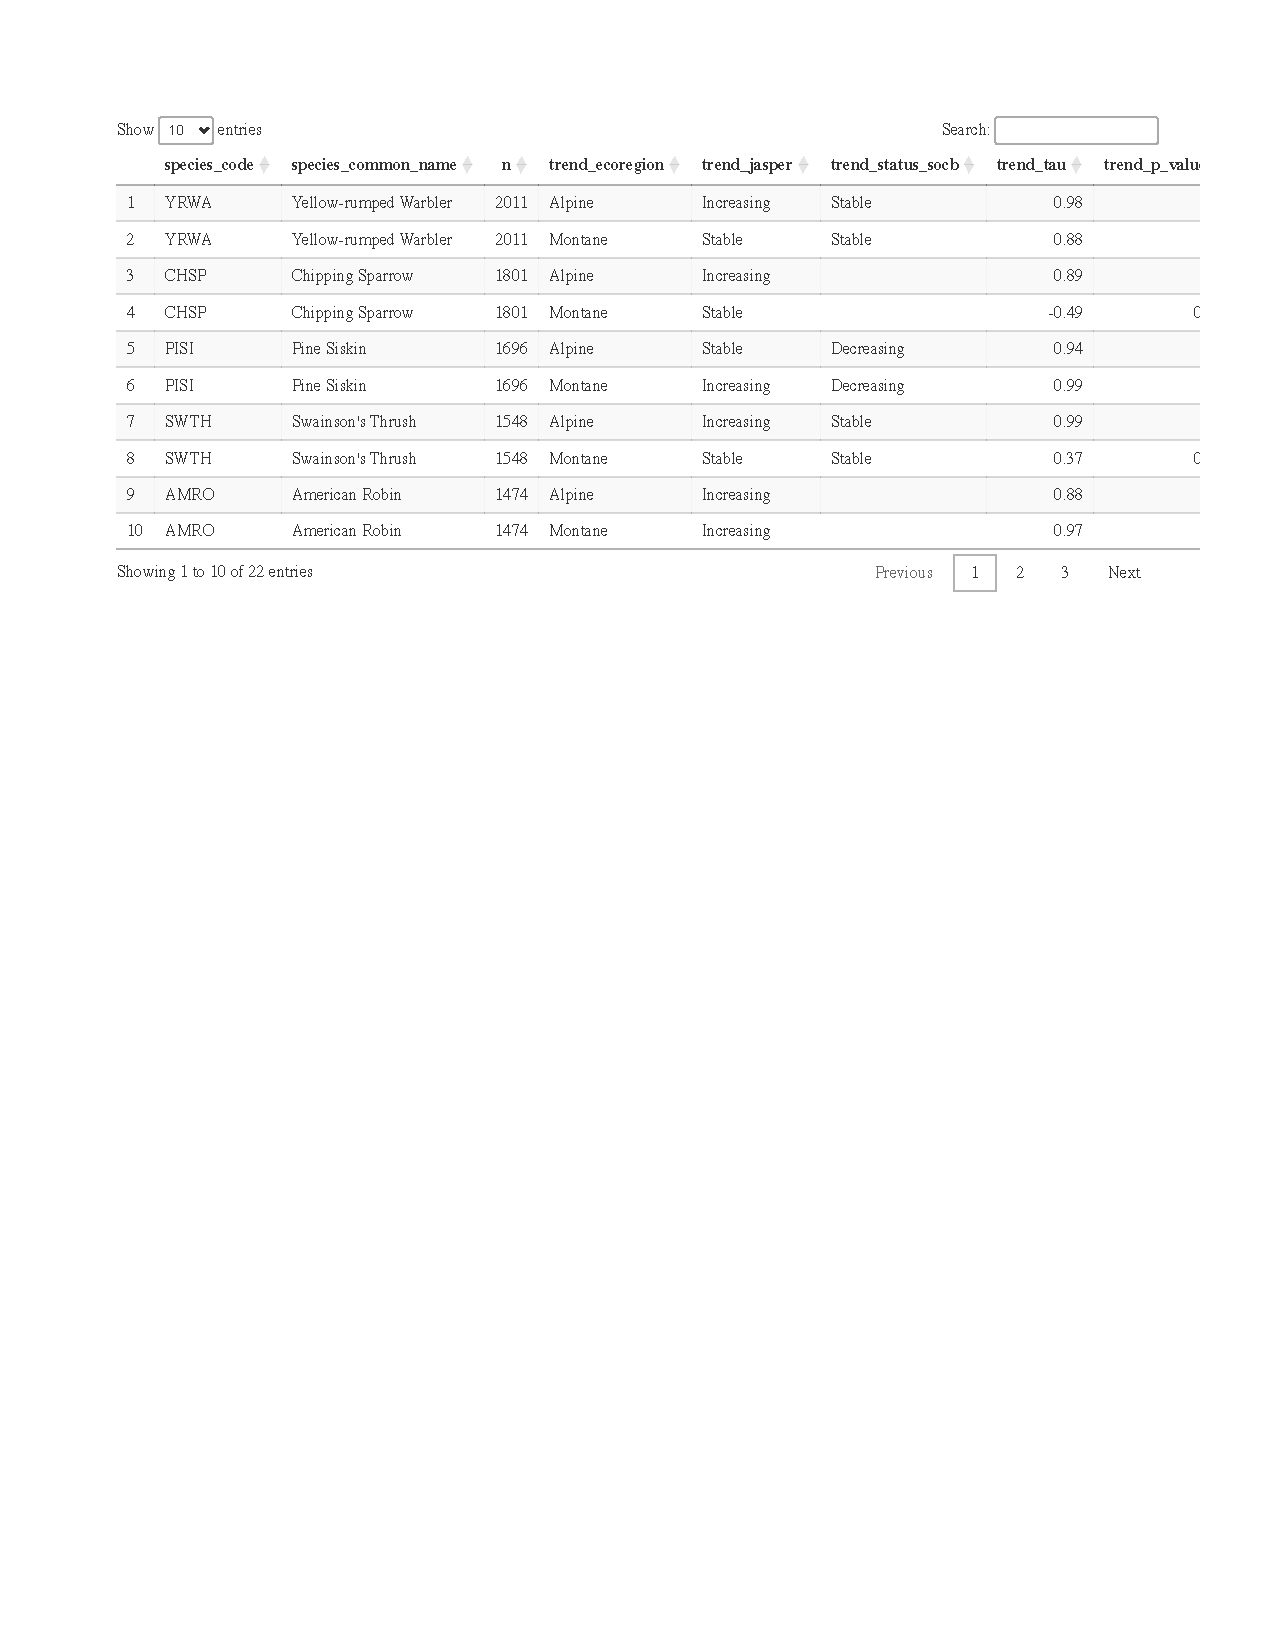
\includegraphics[keepaspectratio]{janp_files/figure-pdf/tbl-trend-1.pdf}}

}

\end{table}%

\begin{figure}

\centering{

\pandocbounded{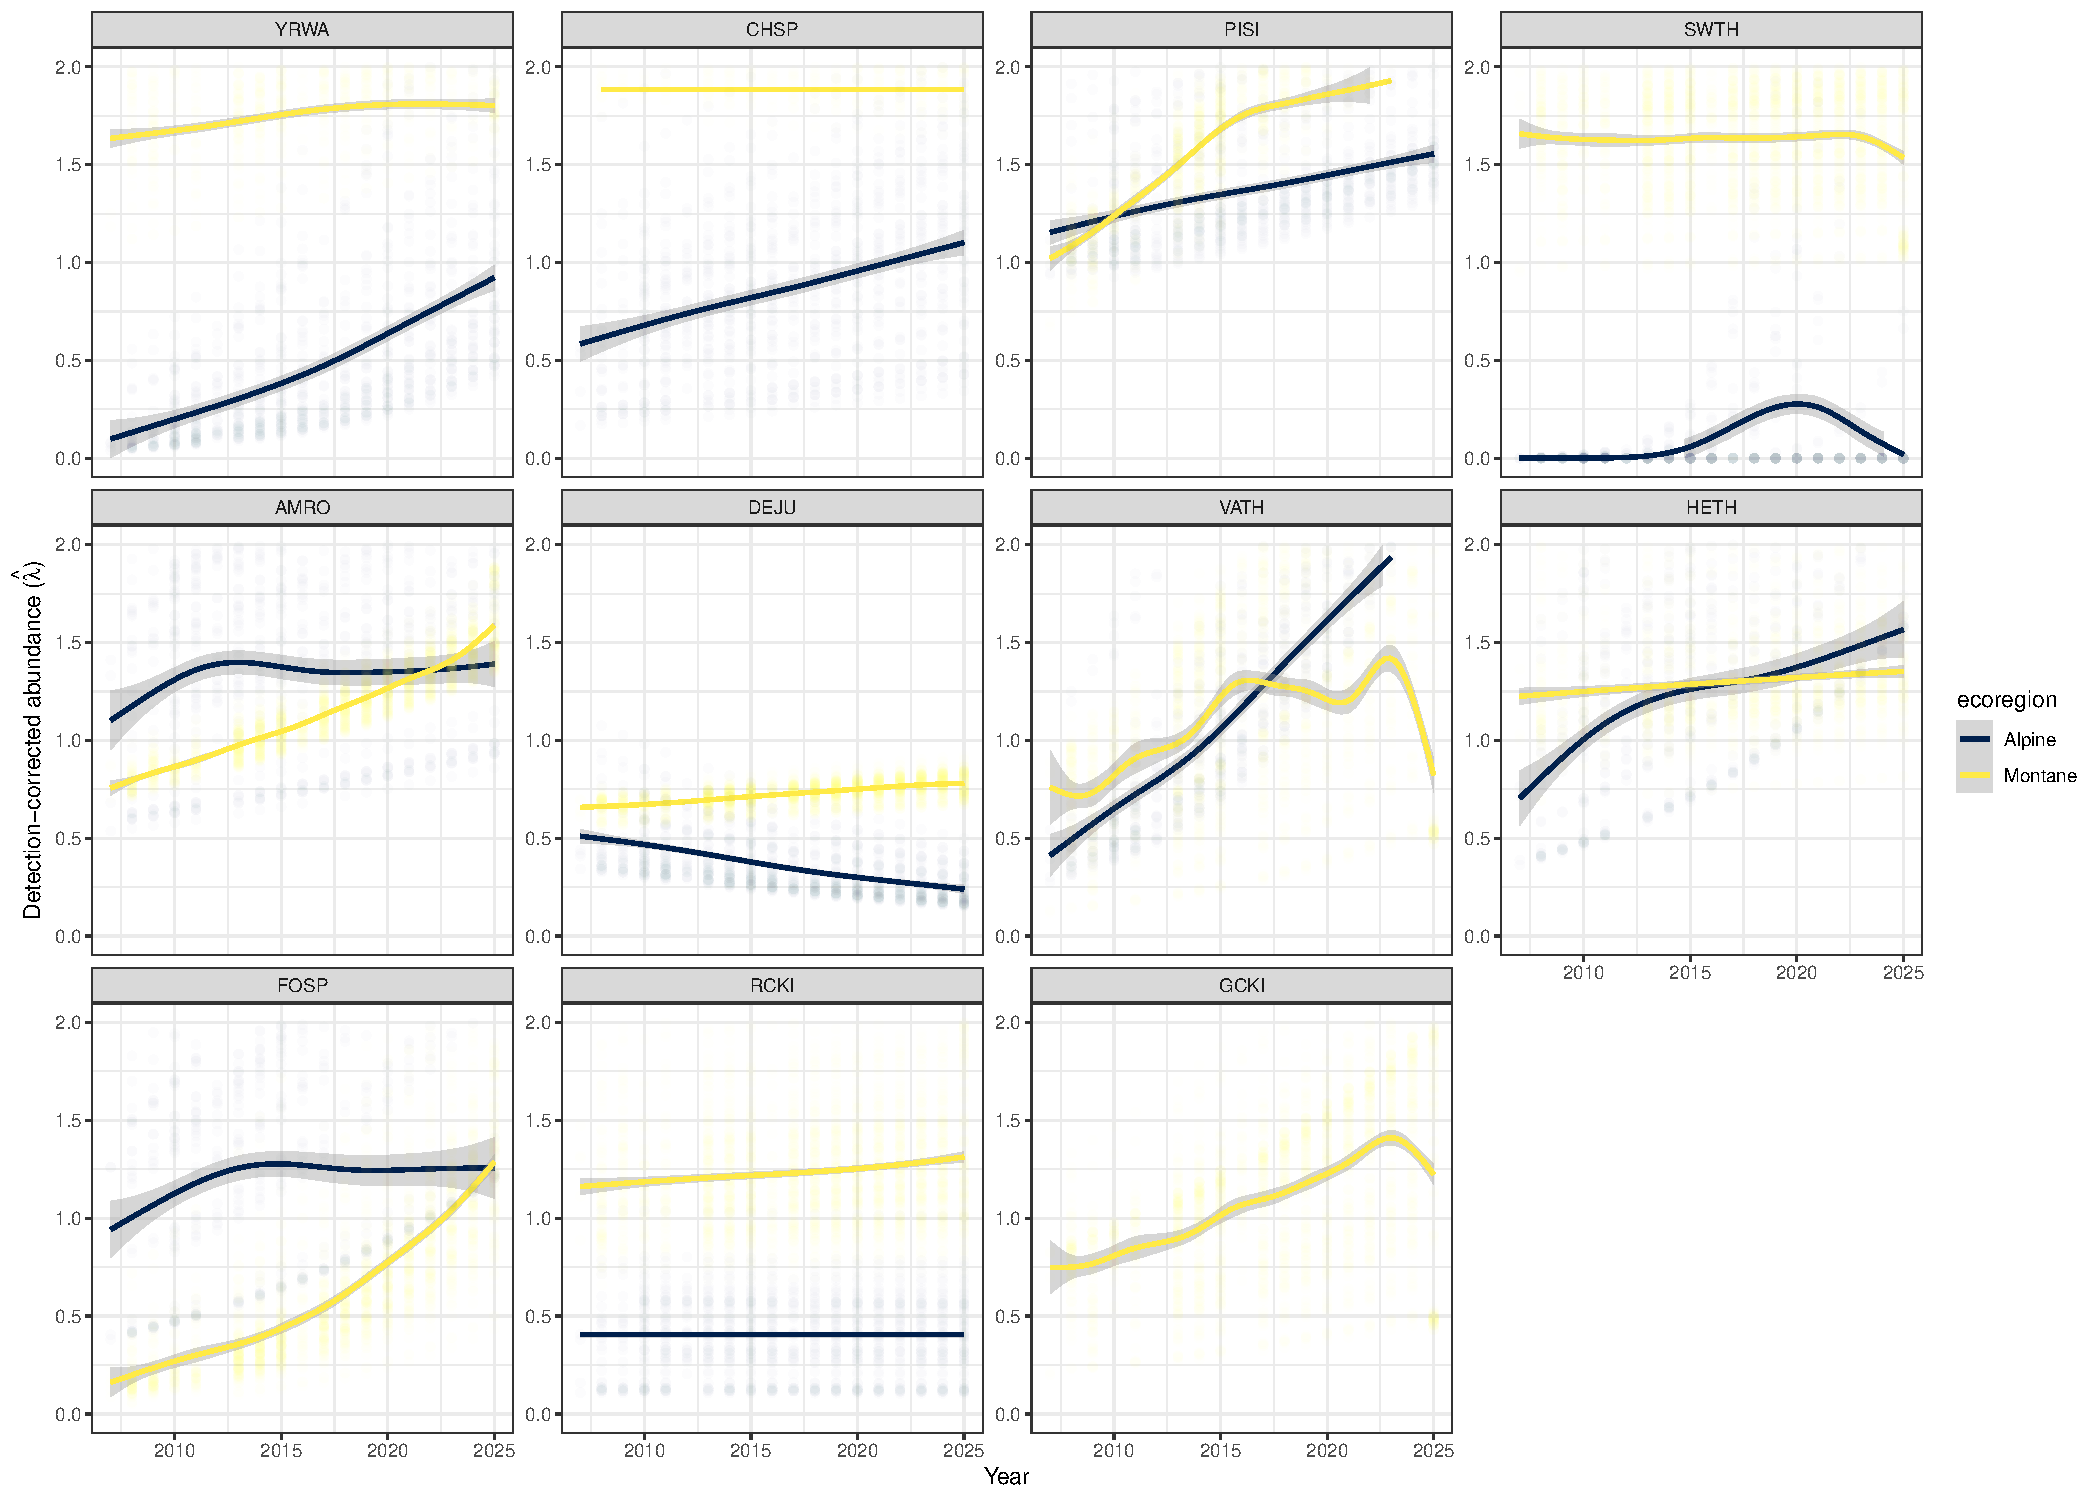
\includegraphics[keepaspectratio]{janp_files/figure-pdf/fig-trend-points-1.pdf}}

}

\caption{\label{fig-trend-points}}

\end{figure}%

\begin{table}

\caption{\label{tbl-trend-2}Summary of trend of species grouped by
ecoregion.}

\centering{

\pandocbounded{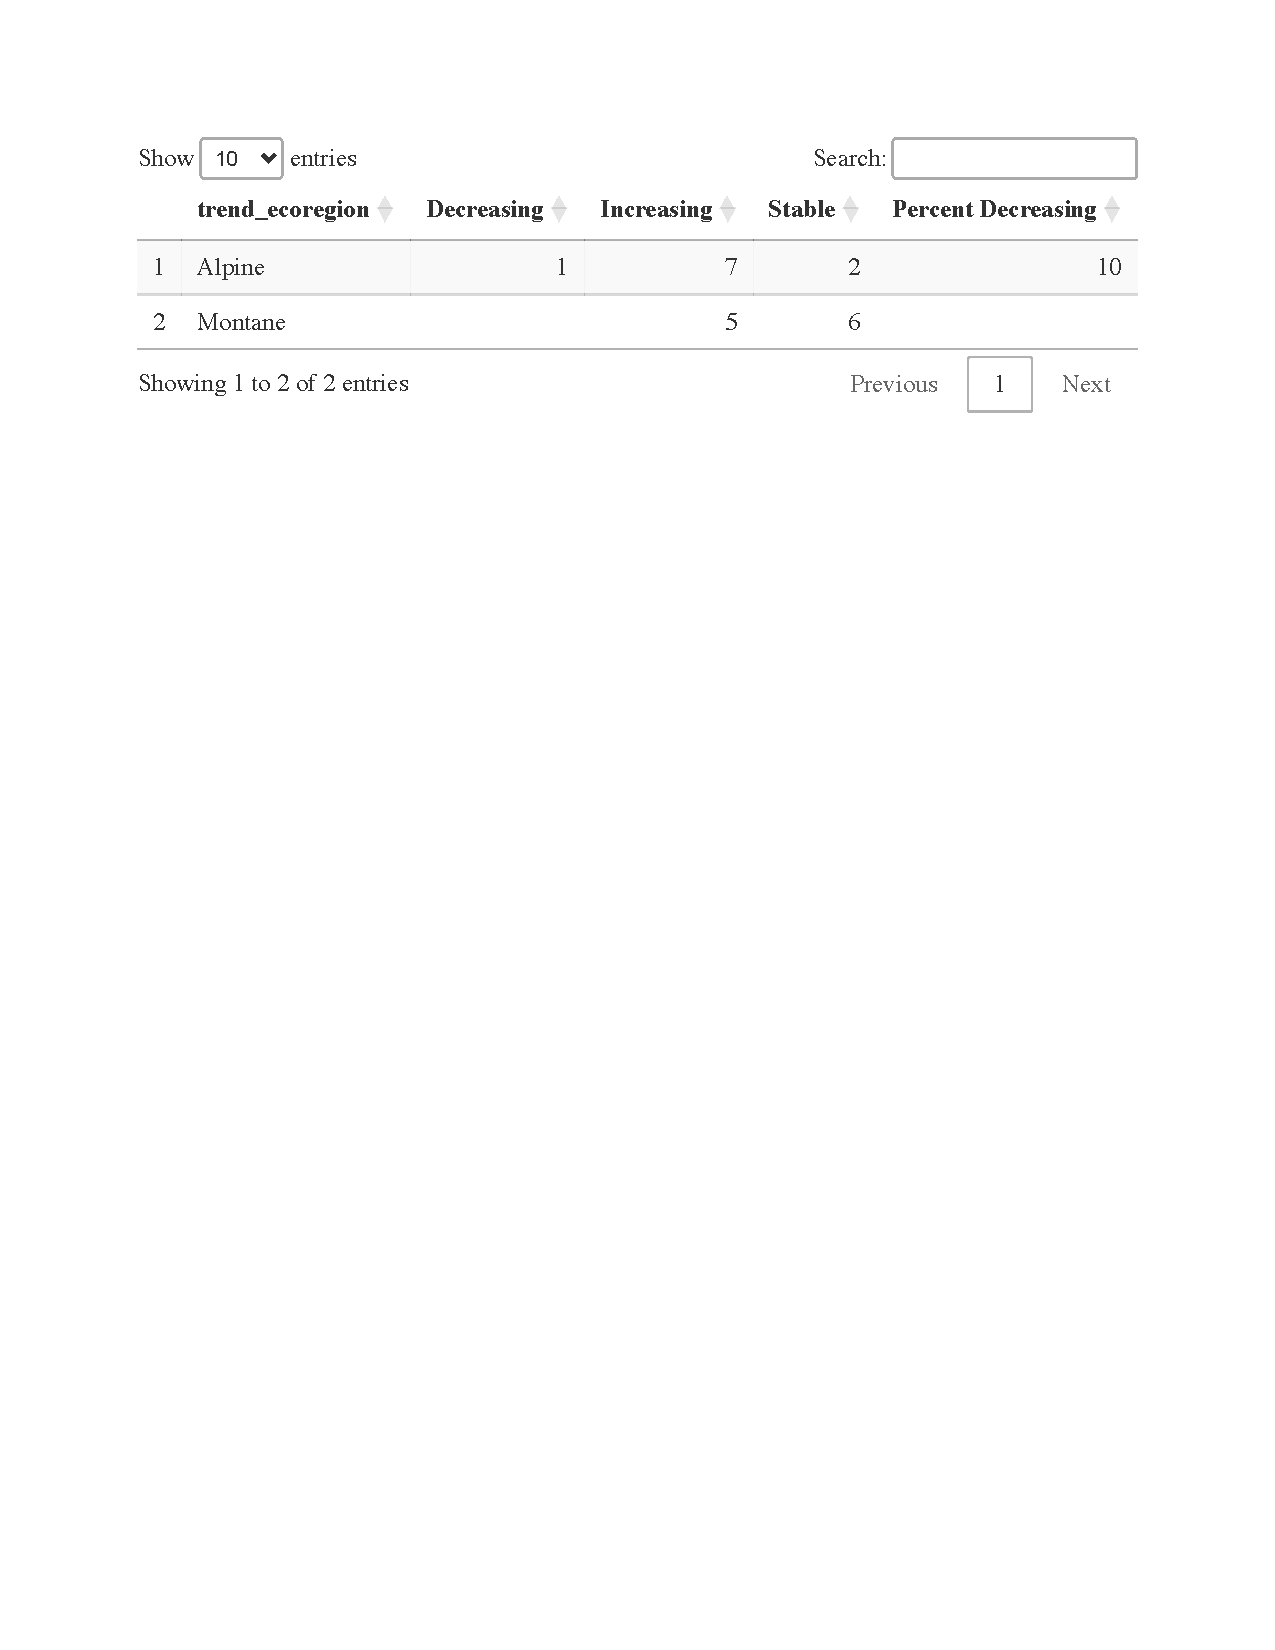
\includegraphics[keepaspectratio]{janp_files/figure-pdf/tbl-trend-2-1.pdf}}

}

\end{table}%

\begin{figure}

\centering{

\pandocbounded{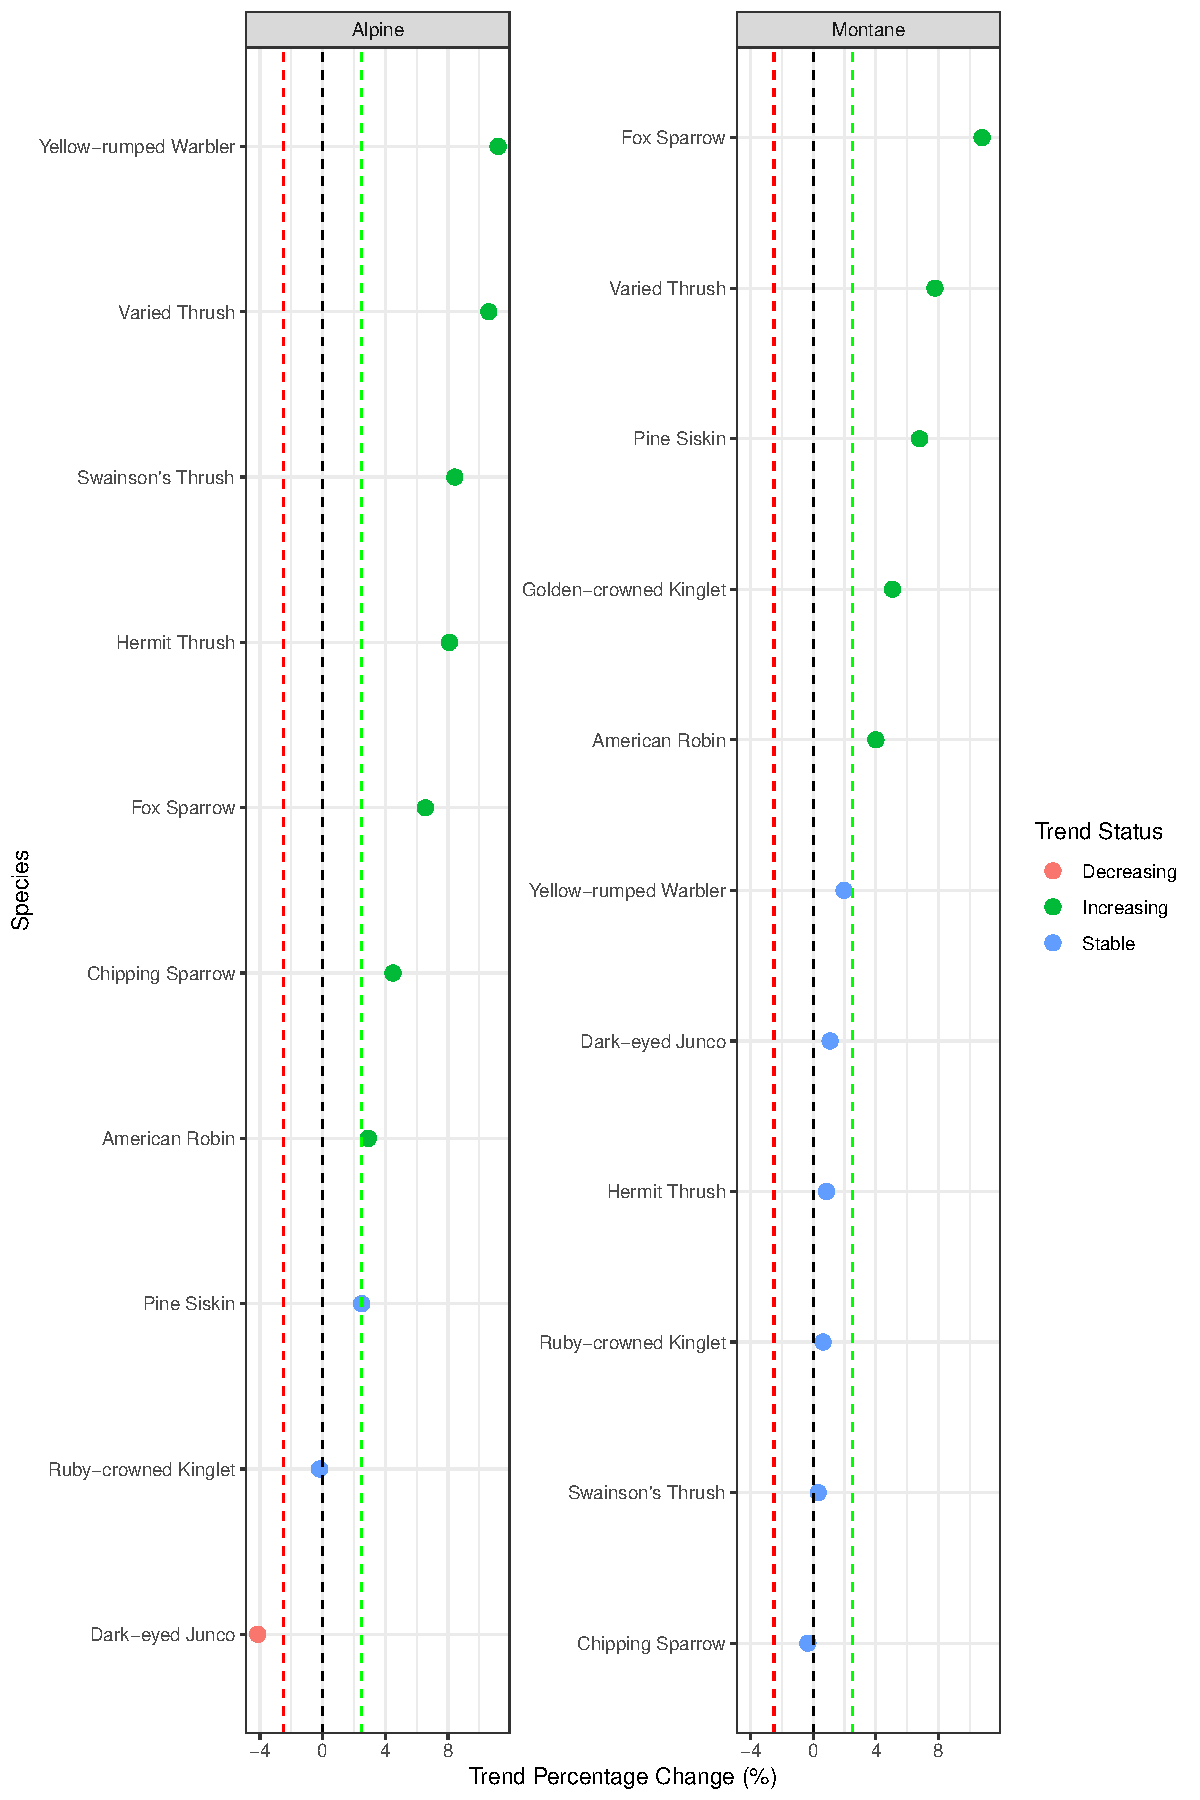
\includegraphics[keepaspectratio]{janp_files/figure-pdf/fig-trend-vert-1.pdf}}

}

\caption{\label{fig-trend-vert}Summary of trend percent change by
species and ecoregion. Colours indicated departure from baseline to
increasing (+2.5\%) or decreasing (-2.5\%) territory.}

\end{figure}%

\section{Discussion and
recommendations}\label{discussion-and-recommendations}

Our analysis confirms that biological phenology, rather than immediate
weather conditions, was the primary driver of species detections in
Jasper National Park. The significant negative relationship between
species richness and both Julian day and survey hour is consistent with
well-established avian activity patterns. The decline in detections
later in the season reflects the cessation of territorial signaling as
breeding concludes (Catchpole \& Slater 2008), while the negative effect
of survey hour captures the waning of the dawn chorus (Robbins 1981).

Contrary to the strong temporal signals, we found that temperature, wind
speed, and sky conditions had weak or non-significant effects on overall
species richness. This lack of a uniform negative response likely
reflects the complexity of bird community responses rather than a total
lack of sensitivity. For instance, Morelli et al.~(2022) found that
weather effects on detectability are highly guild-specific: while wind
negatively affected the detection of insectivores and granivores, it had
no effect on omnivores and was actually associated with increased
detection of granivore-insectivores. In our analysis, these
heterogeneous responses likely offset one another when aggregated into a
single ``Species Richness'' metric. Furthermore, by restricting surveys
to favorable conditions---avoiding high winds and precipitation---the
monitoring program likely minimized the variance attributable to these
factors, ensuring that the observed long-term trends in abundance are
driven by ecological changes rather than artifacts of sampling
conditions.

\phantomsection\label{refs}
\begin{CSLReferences}{1}{0}
\bibitem[\citeproctext]{ref-abrahms2023climate}
Abrahms, Briana, Neil H Carter, TJ Clark-Wolf, Kaitlyn M Gaynor, Erik
Johansson, Alex McInturff, Anna C Nisi, Kasim Rafiq, and Leigh West.
2023. {``Climate Change as a Global Amplifier of Human--Wildlife
Conflict.''} \emph{Nature Climate Change} 13 (3): 224--34.

\bibitem[\citeproctext]{ref-ackleh2010measuring}
Ackleh, Azmy S, Jacoby Carter, Lauren Cole, Tom Nguyen, Jay Monte, and
Claire Pettit. 2010. {``Measuring and Modeling the Seasonal Changes of
an Urban Green Treefrog (Hyla Cinerea) Population.''} \emph{Ecological
Modelling} 221 (2): 281--89.

\bibitem[\citeproctext]{ref-akaike1974}
Akaike, Hirotugu. 1974. {``A New Look at the Statistical Model
Identification.''} \emph{IEEE Transactions on Automatic Control} 19 (6):
716--23. \url{https://doi.org/10.1109/TAC.1974.1100705}.

\bibitem[\citeproctext]{ref-allan2017recent}
Allan, James R, Oscar Venter, Sean Maxwell, Bastian Bertzky, Kendall
Jones, Yichuan Shi, and James EM Watson. 2017. {``Recent Increases in
Human Pressure and Forest Loss Threaten Many Natural World Heritage
Sites.''} \emph{Biological Conservation} 206: 47--55.

\bibitem[\citeproctext]{ref-Anderson2001}
Anderson, Marti J. 2001. {``A New Method for Non-Parametric Multivariate
Analysis of Variance.''} \emph{Austral Ecology} 26 (1): 32--46.
\url{https://doi.org/10.1111/j.1442-9993.2001.01070.pp.x}.

\bibitem[\citeproctext]{ref-bates2015parsimonious}
Bates, Douglas, Reinhold Kliegl, Shravan Vasishth, and Harald Baayen.
2015. {``Parsimonious Mixed Models.''} \emph{arXiv Preprint
arXiv:1506.04967}.

\bibitem[\citeproctext]{ref-bates2015lme4}
Bates, Douglas, Martin Mächler, Ben Bolker, and Steve Walker. 2015.
{``Fitting Linear Mixed-Effects Models Using {lme4}.''} \emph{Journal of
Statistical Software} 67 (1): 1--48.
\url{https://doi.org/10.18637/jss.v067.i01}.

\bibitem[\citeproctext]{ref-birdscanada_stateofbirds_2024}
Birds Canada, and Environment and Climate Change Canada. 2024. {``The
State of Canada's Birds Report.''} Birds Canada; Environment; Climate
Change Canada. \url{https://doi.org/10.71842/8bab-ks08}.

\bibitem[\citeproctext]{ref-vis-scan-amphs}
Cameron, J., A. Crosby, C. Paszkowski, and E. Bayne. 2020. {``Visual
Spectrogram Scanning Paired with an Observation--Confirmation Occupancy
Model Improves the Efficiency and Accuracy of Bioacoustic Anuran
Data.''} \emph{Canadian Journal of Zoology} 98 (11): 733--42.
\url{https://doi.org/10.1139/cjz-2020-0103}.

\bibitem[\citeproctext]{ref-dawood2017spatio}
Dawood, Muhammad. 2017. {``Spatio-Statistical Analysis of Temperature
Fluctuation Using Mann--Kendall and Sen's Slope Approach.''}
\emph{Climate Dynamics} 48 (3): 783--97.

\bibitem[\citeproctext]{ref-devarajan2020multi}
Devarajan, Kadambari, Toni Lyn Morelli, and Simone Tenan. 2020.
{``Multi-Species Occupancy Models: Review, Roadmap, and
Recommendations.''} \emph{Ecography} 43 (11): 1612--24.

\bibitem[\citeproctext]{ref-doser2021trends}
Doser, Jeffrey W, Aaron S Weed, Elise F Zipkin, Kathryn M Miller, and
Andrew O Finley. 2021. {``Trends in Bird Abundance Differ Among
Protected Forests but Not Bird Guilds.''} \emph{Ecological Applications}
31 (6): e02377.

\bibitem[\citeproctext]{ref-fahrig2003effects}
Fahrig, Lenore. 2003. {``Effects of Habitat Fragmentation on
Biodiversity.''} \emph{Annual Review of Ecology, Evolution, and
Systematics} 34 (1): 487--515.

\bibitem[\citeproctext]{ref-farnsworth2002removal}
Farnsworth, George L, Kenneth H Pollock, James D Nichols, Theodore R
Simons, James E Hines, and John R Sauer. 2002. {``A Removal Model for
Estimating Detection Probabilities from Point-Count Surveys.''}
\emph{The Auk} 119 (2): 414--25.

\bibitem[\citeproctext]{ref-gahbauer2022projected}
Gahbauer, Marcel A, Scott R Parker, Joanna X Wu, Cavan Harpur, Brooke L
Bateman, Darroch M Whitaker, Douglas P Tate, Lotem Taylor, and Denis
Lepage. 2022. {``Projected Changes in Bird Assemblages Due to Climate
Change in a Canadian System of Protected Areas.''} \emph{Plos One} 17
(1): e0262116.

\bibitem[\citeproctext]{ref-aru-vs-cams-wolves}
Garland, Laura, Andrew Crosby, Richard Hedley, Stan Boutin, and Erin
Bayne. 2020. {``Acoustic Vs. Photographic Monitoring of Gray Wolves
({Canis lupus}): A Methodological Comparison of Two Passive Monitoring
Techniques.''} \emph{Canadian Journal of Zoology} 98 (3): 219--28.
\url{https://doi.org/10.1139/cjz-2019-0081}.

\bibitem[\citeproctext]{ref-hamed2009}
Hamed, K. H. 2009. {``Exact Distribution of the Mann-Kendall Trend Test
Statistic for Persistent Data.''} \emph{Journal of Hydrology} 365 (1):
86--94. \url{https://doi.org/10.1016/j.jhydrol.2009.01.040}.

\bibitem[\citeproctext]{ref-hamed1998}
Hamed, K. H., and A. Ramachandra Rao. 1998. {``A Modified Mann-Kendall
Trend Test for Autocorrelated Data.''} \emph{Journal of Hydrology} 204
(1): 182--96. \url{https://doi.org/10.1016/S0022-1694(97)00125-X}.

\bibitem[\citeproctext]{ref-handel2004alaska}
Handel, C. M., and M. N. Cady. 2004. {``Alaska Landbird Monitoring
Survey: Protocol for Setting up and Conducting Point Count Surveys.''}
Technical Report 2004-3. Alaska Science Center: U.S. Geological Survey.

\bibitem[\citeproctext]{ref-hanski2011habitat}
Hanski, Ilkka. 2011. {``Habitat Loss, the Dynamics of Biodiversity, and
a Perspective on Conservation.''} \emph{Ambio} 40 (3): 248--55.

\bibitem[\citeproctext]{ref-kendall1975}
Kendall, Maurice G. 1975. \emph{Multivariate Analysis}. Charles Griffin
\& Company Ltd.

\bibitem[\citeproctext]{ref-knight2019classification}
Knight, Elly C, and Erin M Bayne. 2019. {``Classification Threshold and
Training Data Affect the Quality and Utility of Focal Species Data
Processed with Automated Audio-Recognition Software.''}
\emph{Bioacoustics} 28 (6): 539--54.

\bibitem[\citeproctext]{ref-laliberte2010adistance}
Laliberté, Etienne, and Pierre Legendre. 2010. {``A Distance-Based
Framework for Measuring Functional Diversity from Multiple Traits.''}
\emph{Ecology} 91: 299--305.

\bibitem[\citeproctext]{ref-FDpackage}
Laliberté, Etienne, Pierre Legendre, and Bill Shipley. 2014. \emph{FD:
Measuring Functional Diversity from Multiple Traits, and Other Tools for
Functional Ecology}.

\bibitem[\citeproctext]{ref-lemieux2011state}
Lemieux, Christopher J, Thomas J Beechey, Daniel J Scott, and Paul A
Gray. 2011. {``The State of Climate Change Adaptation in Canada's
Protected Areas Sector.''} \emph{The Canadian Geographer/Le G{é}ographe
Canadien} 55 (3): 301--17.

\bibitem[\citeproctext]{ref-Loeb_2015}
Loeb, Susan C., Thomas J. Rodhouse, Laura E. Ellison, Cori L. Lausen,
Jonathan D. Reichard, Kathryn M. Irvine, Thomas E. Ingersoll, et al.
2015. \emph{A Plan for the North American Bat Monitoring Program
(NABat)}. U.S. Department of Agriculture, Forest Service, Southern
Research Station. \url{https://doi.org/10.2737/srs-gtr-208}.

\bibitem[\citeproctext]{ref-Loeb2015}
Loeb, Susan C., Thomas J. Rodhouse, Lee E. Ellison, et al. 2015. \emph{A
Plan for the North American Bat Monitoring Program (NABat)}. Asheville,
NC: U.S. Department of Agriculture, Forest Service, Southern Research
Station. \url{https://doi.org/10.1898/NWN21-10}.

\bibitem[\citeproctext]{ref-lovett2013peepers}
Lovett, Gary M. 2013. {``When Do Peepers Peep? Climate and the Date of
First Calling in the Spring Peeper (Pseudacris Crucifer) in Southeastern
New York State.''} \emph{Northeastern Naturalist} 20 (2): 333--40.

\bibitem[\citeproctext]{ref-occu-fit}
MacKenzie, Darryl I., and Larissa L. Bailey. 2004. {``Assessing the Fit
of Site-Occupancy Models.''} \emph{Journal of Agricultural, Biological,
and Environmental Statistics} 9 (3): 300--318.
\url{http://www.jstor.org/stable/1400484}.

\bibitem[\citeproctext]{ref-imperfect-occu}
MacKenzie, Darryl I., James D. Nichols, James E. Hines, Melinda G.
Knutson, and Alan B. Franklin. 2003. {``ESTIMATING SITE OCCUPANCY,
COLONIZATION, AND LOCAL EXTINCTION WHEN a SPECIES IS DETECTED
IMPERFECTLY.''} \emph{Ecology} 84 (8): 2200--2207.
https://doi.org/\url{https://doi.org/10.1890/02-3090}.

\bibitem[\citeproctext]{ref-mackenzie2002estimating}
MacKenzie, Darryl I, James D Nichols, Gideon B Lachman, Sam Droege, J
Andrew Royle, and Catherine A Langtimm. 2002. {``Estimating Site
Occupancy Rates When Detection Probabilities Are Less Than One.''}
\emph{Ecology} 83 (8): 2248--55.

\bibitem[\citeproctext]{ref-mackenzie2009modeling}
MacKenzie, Darryl I, James D Nichols, Mark E Seamans, and RJ Gutiérrez.
2009. {``Modeling Species Occurrence Dynamics with Multiple States and
Imperfect Detection.''} \emph{Ecology} 90 (3): 823--35.

\bibitem[\citeproctext]{ref-MacPhail2026_avian}
MacPhail, Alexander G., Corrina Copp, Erin Bayne, Charles Francis,
Michael Packer, Chad Klassen, Kevin Kelly, et al. 2026. {``WildTrax: A
Platform for the Management, Storage, Processing, Sharing and Discovery
of Avian Data.''}

\bibitem[\citeproctext]{ref-mann1945non}
Mann, H. B. 1945a. {``Non-Parametric Tests Against Trend.''}
\emph{Econometrica: Journal of the Econometric Society} 13 (3): 245--59.

\bibitem[\citeproctext]{ref-mann1945}
---------. 1945b. {``Nonparametric Tests Against Trend.''}
\emph{Econometrica} 13 (3): 245--59.
\url{https://doi.org/10.1017/CBO9781107415324.004}.

\bibitem[\citeproctext]{ref-mantyka2012interactions}
Mantyka-pringle, Chrystal S, Tara G Martin, and Jonathan R Rhodes. 2012.
{``Interactions Between Climate and Habitat Loss Effects on
Biodiversity: A Systematic Review and Meta-Analysis.''} \emph{Global
Change Biology} 18 (4): 1239--52.

\bibitem[\citeproctext]{ref-segmented2008}
Muggeo, Vito M. R. 2008. {``Segmented: An r Package to Fit Regression
Models with Broken-Line Relationships.''} \emph{R News} 8 (1): 20--25.
\url{https://cran.r-project.org/doc/Rnews/}.

\bibitem[\citeproctext]{ref-oksanen2010canonical}
Oksanen, Jari, Frank G Blanchet, Roeland Kindt, Pierre Legendre, Peter R
Minchin, Robert B O'Hara, Gavin L Simpson, et al. 2010. {``Canonical
Analysis of Principal Coordinates: A Useful Method of Constrained
Ordination for Ecology.''} \emph{Ecology} 92 (3): 597--611.
\url{https://doi.org/10.1890/10-0340.1}.

\bibitem[\citeproctext]{ref-vegan2025}
Oksanen, Jari, Gavin L. Simpson, F. Guillaume Blanchet, Roeland Kindt,
Pierre Legendre, Peter R. Minchin, R. B. O'Hara, et al. 2025.
\emph{Vegan: Community Ecology Package}.
\url{https://vegandevs.github.io/vegan/}.

\bibitem[\citeproctext]{ref-onoz2012}
Önöz, B., and M. Bayazit. 2012. {``The Power of Statistical Tests for
Trend Detection.''} \emph{Hydrological Processes} 26 (17): 2809--14.
\url{https://doi.org/10.1002/hyp.8438}.

\bibitem[\citeproctext]{ref-pacifici2014guidelines}
Pacifici, Krishna, Elise F Zipkin, Jaime A Collazo, Julissa I Irizarry,
and Amielle DeWan. 2014. {``Guidelines for a Priori Grouping of Species
in Hierarchical Community Models.''} \emph{Ecology and Evolution} 4 (7):
877--88.

\bibitem[\citeproctext]{ref-Petrikeev2019analysis}
Petrikeev, Michael. 2019. {``Forest Breeding Bird Abundance and
Composition, Kluane National Park Reserve.''}

\bibitem[\citeproctext]{ref-prowse2021optimising}
Prowse, Thomas AA, Patrick J O'Connor, Stuart J Collard, Kristian J
Peters, and Hugh P Possingham. 2021. {``Optimising Monitoring for Trend
Detection After 16 Years of Woodland-Bird Surveys.''} \emph{Journal of
Applied Ecology} 58 (5): 1090--100.

\bibitem[\citeproctext]{ref-rao1982diversity}
Rao, C. R. 1982. {``Diversity and Dissimilarity Coefficients: A Unified
Approach.''} \emph{Theoretical Population Biology} 21 (1): 24--43.

\bibitem[\citeproctext]{ref-Rao1964}
Rao, C. Radhakrishna. 1964. {``The Use and Interpretation of Principal
Component Analysis in Applied Research.''} \emph{Sankhya: The Indian
Journal of Statistics, Series A} 26 (4): 329--58.

\bibitem[\citeproctext]{ref-Reichert2018}
Reichert, B., C. Lausen, S. Loeb, et al. 2018. \emph{A Guide to
Processing Bat Acoustic Data for the North American Bat Monitoring
Program (NABat)}. U.S. Geological Survey.
\url{https://doi.org/10.1898/NWN21-10}.

\bibitem[\citeproctext]{ref-reichert2018guide}
Reichert, Brian, Cori Lausen, Susan Loeb, Ted Weller, Ryan Allen, Eric
Britzke, Tara Hohoff, et al. 2018. {``A Guide to Processing Bat Acoustic
Data for the North American Bat Monitoring Program (NABat).''} US
Geological Survey.

\bibitem[\citeproctext]{ref-rosenberg2019decline}
Rosenberg, Kenneth V, Adriaan M Dokter, Peter J Blancher, John R Sauer,
Adam C Smith, Paul A Smith, Jessica C Stanton, et al. 2019. {``Decline
of the North American Avifauna.''} \emph{Science} 366 (6461): 120--24.

\bibitem[\citeproctext]{ref-sattar2021review}
Sattar, Q, ME Maqbool, R Ehsan, S Akhtar, Q Sattar, ME Maqbool, R Ehsan,
and S Akhtar. 2021. {``Review on Climate Change and Its Effect on
Wildlife and Ecosystem.''} \emph{Open J Environ Biol} 6 (1): 008--14.

\bibitem[\citeproctext]{ref-sedgwick2012pearson}
Sedgwick, Philip. 2012. {``Pearson's Correlation Coefficient.''}
\emph{Bmj} 345.

\bibitem[\citeproctext]{ref-sen1968}
Sen, P. K. 1968. {``Estimates of the Regression Coefficient Based on
Kendall's Tau.''} \emph{Journal of the American Statistical Association}
63 (324): 1379--89. \url{https://doi.org/10.2307/2285891}.

\bibitem[\citeproctext]{ref-Sen01121968}
Sen, Pranab Kumar. 1968. {``Estimates of the Regression Coefficient
Based on Kendall's Tau.''} \emph{Journal of the American Statistical
Association} 63 (324): 1379--89.
\url{https://doi.org/10.1080/01621459.1968.10480934}.

\bibitem[\citeproctext]{ref-shannon1948mathematical}
Shannon, Claude Elwood. 1948. {``A Mathematical Theory of
Communication.''} \emph{The Bell System Technical Journal} 27 (3):
379--423.

\bibitem[\citeproctext]{ref-aru-overview}
Shonfield, Julia, and Erin M Bayne. 2017. {``Autonomous Recording Units
in Avian Ecological Research: Current Use and Future Applications.''}
\emph{Avian Conservation \& Ecology} 12 (1).

\bibitem[\citeproctext]{ref-shonfield2018utility}
Shonfield, Julia, Sarah Heemskerk, and Erin M Bayne. 2018. {``Utility of
Automated Species Recognition for Acoustic Monitoring of Owls.''}
\emph{Journal of Raptor Research} 52 (1): 42--55.

\bibitem[\citeproctext]{ref-Slough2022}
Slough, B., C. Lausen, B. Paterson, et al. 2022. {``New Records about
the Diversity, Distribution, and Seasonal Activity Patterns by Bats in
Yukon and Northwestern British Columbia.''} \emph{Northwest Naturalist}
103: 162--82. \url{https://doi.org/10.1898/NWN21-10}.

\bibitem[\citeproctext]{ref-slough2023little}
Slough, Brian G, Donald G Reid, Dafna S Schultz, and Maria C-Y Leung.
2023. {``Little Brown Bat Activity Patterns and Conservation
Implications in Agricultural Landscapes in Boreal Yukon, Canada.''}
\emph{Ecosphere} 14 (3): e4446.

\bibitem[\citeproctext]{ref-smith2015change}
Smith, Adam C, Marie-Anne R Hudson, Constance M Downes, and Charles M
Francis. 2015. {``Change Points in the Population Trends of
Aerial-Insectivorous Birds in North America: Synchronized in Time Across
Species and Regions.''} \emph{PloS One} 10 (7): e0130768.

\bibitem[\citeproctext]{ref-Solick2022}
Solick, Daniel I. 2022. {``Bat Acoustic Species-Pair Matrix for Western
u.s./Canada.''} Colorado: Vesper Bat Detection Services.

\bibitem[\citeproctext]{ref-solick2022coat}
Solick, Donald I, and Robert MR Barclay. 2022. {``Coat Color of Western
Long-Eared Bats (Myotis Evotis) Living in Different Environments: A Test
of Gloger's Rule.''} \emph{Northwestern Naturalist} 103 (2): 183--89.

\bibitem[\citeproctext]{ref-solymos2012conditional}
Sólymos, Péter, Subhash Lele, and Erin Bayne. 2012. {``Conditional
Likelihood Approach for Analyzing Single Visit Abundance Survey Data in
the Presence of Zero Inflation and Detection Error.''}
\emph{Environmetrics} 23 (2): 197--205.
https://doi.org/\url{https://doi.org/10.1002/env.1149}.

\bibitem[\citeproctext]{ref-solymos2013calibrating}
Sólymos, Péter, Steven M Matsuoka, Erin M Bayne, Subhash R Lele,
Patricia Fontaine, Steve G Cumming, Diana Stralberg, Fiona KA
Schmiegelow, and Samantha J Song. 2013. {``Calibrating Indices of Avian
Density from Non-Standardized Survey Data: Making the Most of a Messy
Situation.''} \emph{Methods in Ecology and Evolution} 4 (11): 1047--58.

\bibitem[\citeproctext]{ref-time-removal}
Sólymos, Péter, Steven M. Matsuoka, Steven G. Cumming, Diana Stralberg,
Patricia Fontaine, Fiona K. A. Schmiegelow, Samantha J. Song, and Erin
M. Bayne. 2018. {``{Evaluating time-removal models for estimating
availability of boreal birds during point count surveys: Sample size
requirements and model complexity}.''} \emph{The Condor} 120 (4):
765--86. \url{https://doi.org/10.1650/CONDOR-18-32.1}.

\bibitem[\citeproctext]{ref-Szewczak2024western_na_bat_acoustic_table}
Sonobat. n.d. {``Western North America Bat Acoustic Table.''}
\url{https://sonobat.com/download/Western_NA_Bat_Acoustic_Table.pdf}.

\bibitem[\citeproctext]{ref-lots-of-pam}
Sugai, Larissa Sayuri Moreira, Thiago Sanna Freire Silva, Jr Ribeiro
José Wagner, and Diego Llusia. 2018. {``{Terrestrial Passive Acoustic
Monitoring: Review and Perspectives}.''} \emph{BioScience} 69 (1):
15--25. \url{https://doi.org/10.1093/biosci/biy147}.

\bibitem[\citeproctext]{ref-birds6010014}
Suthar, Akshit R., Alan R. Biggs, and James T. Anderson. 2025. {``A
Decadal Change in Shorebird Populations in Response to Temperature,
Wind, and Precipitation at Hilton Head Island, South Carolina, USA.''}
\emph{Birds} 6 (1). \url{https://www.mdpi.com/2673-6004/6/1/14}.

\bibitem[\citeproctext]{ref-Szewczak2018}
Szewczak, Joe. 2018. {``Acoustic Features of Western US Bats.''} Arcata,
California: Humboldt State University.

\bibitem[\citeproctext]{ref-arus-mics}
Turgeon, Patrick, Steven L. Van Wilgenburg, and Kiel L. Drake. 2017.
{``Microphone Variability and Degradation: Implications for Monitoring
Programs Employing Autonomous Recording Units.''} \emph{Avian
Conservation and Ecology} 12.
\url{https://api.semanticscholar.org/CorpusID:89959184}.

\bibitem[\citeproctext]{ref-all-the-scans}
Ware, Lena, C. Lisa Mahon, Logan McLeod, and Jean-François Jetté. 2023.
{``Artificial Intelligence (BirdNET) Supplements Manual Methods to
Maximize Bird Species Richness from Acoustic Data Sets Generated from
Regional Monitoring.''} \emph{Canadian Journal of Zoology} 101 (12):
1031--51. \url{https://doi.org/10.1139/cjz-2023-0044}.

\bibitem[\citeproctext]{ref-yip2025contributions}
Yip, Daniel A, Elly C Knight, and Erin M Bayne. 2025. {``Contributions
of Environmental Conditions and Sound Characteristics to Differences in
Perceptibility: Recommendations for Passive Acoustic Monitoring.''}
\emph{Ornithological Applications}, September, duaf059.
\url{https://doi.org/10.1093/ornithapp/duaf059}.

\end{CSLReferences}




\end{document}
